\documentclass[../tesis_main_file.tex]{subfiles}
\begin{document}
\onlyinsubfile{\graphicspath{ {../figuras/} }}
\onlyinsubfile{\pagenumbering{arabic}}
\onlyinsubfile{\chapter{Inestabilidad de dos corrientes.}}
\section{Introducción}
Este capítulo habla de las interacciones entre un conjunto de partículas y una onda. En partícular, el intercambio de energía que ocurre durante la interacción.\\
Para tratar el tema de inestabilidades se mostrará primero que frecuencias complejas pueden aparecer en el plasma si se tiene un arreglo de haces de partículas adecuado \cite{bellan2008fundamentals}.
\section{Relación de dispersión}
El tratamiento inicial se hará desde la perspectiva de fluidos. Se parte entonces de las siguientes ecuaciones:
\begin{equation}
\label{cont_nl}
\frac{\partial n_{\sigma}}{\partial t} + \overrightarrow{\nabla} \cdot n_{\sigma}\overrightarrow{\textbf{u}}_{\sigma}=0
\end{equation}
\begin{equation}
\label{eq_movimiento_nl}
n_{\sigma}m_{\sigma}\frac{d\overrightarrow{\textbf{u}}_{\sigma}}{dt}= n_{\sigma}q_{\sigma}(\overrightarrow{\textbf{E}} + \overrightarrow{\textbf{u}}_{\sigma} \times \overrightarrow{\textbf{B}}) - \nabla P_{\sigma} - \textbf{R}_{\sigma \alpha}
\end{equation}
\begin{equation}
\label{poisson_nl}
\nabla ^2 \Phi = -\frac{1}{\epsilon_0}\sum _{\sigma}q_{\sigma} n_{\sigma}
\end{equation}
Las cuales son respectivamente la ecuación de continuidad, movimiento y Poisson para cada especie. Al tratarse del caso electróstatico la ecuación \ref{eq_movimiento_nl} se puede reducir a la siguiente forma:
\begin{equation}
\label{eq_mov_simpl_nl}
n_{\sigma}m_{\sigma}\frac{d\overrightarrow{\textbf{u}}_{\sigma}}{dt}= n_{\sigma}q_{\sigma} \overrightarrow{\textbf{E}}
\end{equation}
Con $\overrightarrow{\textbf{E}} = - {\overrightarrow\nabla} \Phi$. Y donde se han despreciado los términos de aceleración debido al campo magnético (puesto que ese término es cero para modos longitudinales), la presión y a la fuerza de fricción debida a colisiones. Además, se tiene $d/dt \equiv \partial / \partial t + \overrightarrow{\textbf{u}}_{\sigma} \cdot \overrightarrow{\nabla}$, la cual se le conoce como la derivada convectiva.\\
%Los términos $\nabla P_{\sigma}$ y $\textbf{R}_{\sigma \alpha}$ se refieren a la presión y a la fuerza de fricción resultante de las colisiones entre las especies $\sigma$ y $\alpha$ respectivamente.\\
El siguiente paso entonces es introducir un método que permita ver el comportamiento de las ondas longitudinales en el  plasma debido a cada una de las especies. Dicho método se le conoce como análisis lineal y el procedimiento es el siguiente:
\begin{itemize}
\item Se reduce el sistema a un simple conjunto de ecuaciones que describan su comportamiento.
\item Se determina una solución de equilibrio para las ecuaciones y a las cantidades de equilibrio se les designa con el subíndice 0, indicando que son cantidades de orden cero.
\item Si $\lbrace f(\textbf{x},t), g(\textbf{x},t),h(\textbf{x},t),...\rbrace$ es el conjunto de las variables dependientes y se le agrega una perturbación a una de las variables, entonces al resolver el sistema de ecuaciones se obtendrá la respuesta de las otras variables a la perturbación. Supongasé que se le agrega una perturbación $\epsilon f_1$ a la variable $f$, con $\epsilon \ll 1$ entonces se tiene:
\begin{equation*}
f = f_0 + \epsilon f_1
\end{equation*}
El sistema entonces da la dependencia funcional de las otras variables, por ejemplo $g = g(f) = g(f_0 + \epsilon f_1)$. Dado que ésta dependencia por lo general es no lineal la expansión de Taylor da $g = g_0 + \epsilon g_1 + \epsilon^2 g_2 + \epsilon^3 g_3 +...$ Si se considera a las epsilons como coeficientes implícitos las variables se pueden escribir entonces como:
$$
\begin{array}{lllllllll}
f &= &f_0 &+ &f_1 \\
g &= &g_0 &+ &g_1 &+ &g_2 &+ &...\\
h &= &h_0 &+ &h_1 &+ &h_2 &+ &...
\end{array}
$$
\item Se reescriben entonces las ecuaciones del sistema con las variables expandidas a primer orden y se discriminan los términos de segundo orden resultantes, así como también haciendo uso de las soluciones de equilibrio para simplificar las expresiones.
\end{itemize}
Para el caso de la ecuación de continuidad se tiene entonces:
\begin{equation}
\frac{\partial (n_{\sigma 0} + n_{\sigma 1})}{\partial t} + \overrightarrow{\nabla} \cdot [(n_{\sigma 0}+n_{\sigma 1})(\overrightarrow{\textbf{u}}_{\sigma 0} + \overrightarrow{\textbf{u}}_{\sigma 1})]=0
\end{equation}
Donde la solución de equiibrio es:
\begin{equation}
\frac{\partial n_{\sigma 0}}{\partial t} + \overrightarrow{\nabla} \cdot n_{\sigma 0}\overrightarrow{\textbf{u}}_{\sigma 0}=0
\end{equation}
Lo que da:
\begin{equation}
\frac{\partial n_{\sigma 1}}{\partial t}+ \overrightarrow{\nabla} \cdot (n_{\sigma 1} \overrightarrow{\textbf{u}}_{\sigma 0} + n_{\sigma 0} \overrightarrow{\textbf{u}}_{\sigma 1} + n_{\sigma 1} \overrightarrow{\textbf{u}}_{\sigma 1}) =0
\end{equation}
El término $n_1 \overrightarrow{\textbf{u}}_1$ es de segundo orden y por lo tanto se descarta. Con lo que la ecuación de continuidad linealizada es:
\begin{equation}
\label{cont_lin}
\frac{\partial n_{\sigma 1}}{\partial t}+ \overrightarrow{\nabla} \cdot (n_{\sigma 1} \overrightarrow{\textbf{u}}_{\sigma 0} + n_{\sigma 0} \overrightarrow{\textbf{u}}_{\sigma 1}) =0
\end{equation}
De manera similar, las ecuaciones de movimiento y de Poisson son linealizadas para dar:
\begin{equation}
\label{eq_mov_lin}
\frac{\partial \overrightarrow{\textbf{u}}_{\sigma 1}}{\partial t} + \overrightarrow{\textbf{u}}_{\sigma 0} \cdot \overrightarrow{\nabla}\overrightarrow{\textbf{u}}_{\sigma 1} = - \frac{q_{\sigma}}{m_{\sigma}} \overrightarrow{\nabla}\Phi _1
\end{equation}
\begin{equation}
\label{poisson_lin}
\nabla ^2 \Phi _1 = -\frac{1}{\epsilon_0}\sum _{\sigma}q_{\sigma} n_{\sigma 1}
\end{equation}
Recordando que lo que se quiere estudiar está en el marco de ondas longitudinales en el plasma se considera que la perturbación lineal es un modo de Fourier. Por lo cual las variables cambian de la misma manera en la que lo haría exp ($i \overrightarrow{\textbf{k}} \cdot \overrightarrow{\textbf{x}} - i \omega t $), es decir $\overrightarrow{\nabla} \rightarrow i\overrightarrow{\textbf{k}}$ y $\partial / \partial t \rightarrow -i \omega$ por lo que las ecuaciones \ref{cont_lin}, \ref{eq_mov_lin} y \ref{poisson_lin} se pueden reescribir como:
\begin{equation}
\label{cont_fourier}
 -i \omega n_{\sigma 1}+ i\overrightarrow{\textbf{k}} \cdot (n_{\sigma 1} \overrightarrow{\textbf{u}}_{\sigma 0} + n_{\sigma 0} \overrightarrow{\textbf{u}}_{\sigma 1}) =0
\end{equation}
\begin{equation}
\label{eq_mov_fourier}
-i \omega \overrightarrow{\textbf{u}}_{\sigma 1} + \overrightarrow{\textbf{u}}_{\sigma 0} \cdot i \overrightarrow{\textbf{k}}\overrightarrow{\textbf{u}}_{\sigma 1} = - \frac{i q_{\sigma}}{m_{\sigma}} \overrightarrow{\textbf{k}}\Phi _1
\end{equation}
\begin{equation}
\label{poisson_fourier}
-k^2 \Phi _1 = -\frac{1}{\epsilon_0}\sum _{\sigma}q_{\sigma} n_{\sigma 1}
\end{equation}
Si se fatoriza el término de primer orden de la velocidad en la ecuación de movimiento se obtiene:
\begin{equation}
\label{U1}
\overrightarrow{\textbf{u}}_{\sigma 1} = \frac{- i q_{\sigma} k \Phi _1}{m_{\sigma}(-i \omega + \overrightarrow{\textbf{u}}_{\sigma 0} \cdot i \overrightarrow{\textbf{k}})}
\end{equation}
Al sustituir \ref{U1} en \ref{cont_fourier} se obtiene:
\begin{equation}
n_{\sigma 1} = n_{\sigma 0}\frac{k^2 q_{\sigma} \Phi _1  }{m_{\sigma}(\omega - \overrightarrow{\textbf{u}}_{\sigma 0} \cdot \overrightarrow{\textbf{k}})^2 }
\end{equation}
La cual a su vez se sustituye en \ref{poisson_fourier} y recordando que $\omega_{p \sigma}^2 = q_{\sigma}^2 n_{\sigma 0} / m_{\sigma} \epsilon_0$ se llega a:
\begin{equation}
\label{eq_dispersion}
1 = \sum_{\sigma} \frac{\omega_{p \sigma}^2}{(\omega - \overrightarrow{\textbf{u}}_{\sigma 0} \cdot \overrightarrow{\textbf{k}})^2}
\end{equation}
A la expresión resultante se le conoce como la relación de dispersión. Se tienen entonces las herramientas necesarias para este primer estudio de inestabilidades en un plasma para distintas configuraciones de haces.\\
Debido a que la ecuación \ref{eq_dispersion} parte de la ecuación de Poisson se puede inferir que la relación de dispersión es equivalente a una expresión para la permitividad eléctrica. Para ver esto se recuerda que
$\nabla ^2 \Phi _1 = - \nabla \cdot \overrightarrow{\textbf{E}}$ o en este caso $-k^2 \Phi _1 = -i \overrightarrow{\textbf{k}} \cdot \overrightarrow{\textbf{E}}$ por lo que se puede escribir:
\begin{equation}
-i \overrightarrow{\textbf{k}} \cdot \overrightarrow{\textbf{E}} = - \sum \frac{\omega_{p \sigma}^2 k^2 \Phi _1}{(\omega - \overrightarrow{\textbf{u}}_{\sigma 0} \cdot \overrightarrow{\textbf{k}})^2} = - \sum \frac{\omega_{p \sigma}^2 (i \overrightarrow{\textbf{k}} \cdot \overrightarrow{\textbf{E}})}{(\omega - \overrightarrow{\textbf{u}}_{\sigma 0} \cdot \overrightarrow{\textbf{k}})^2}
\end{equation}
Factorizando términos se llega a:
\begin{equation}
\label{eq:gauss_dilectric_omega}
i \overrightarrow{\textbf{k}} \cdot \overrightarrow{\textbf{E}} \left( 1 - \sum \frac{\omega_{p \sigma}^2 }{(\omega - \overrightarrow{\textbf{u}}_{\sigma 0} \cdot \overrightarrow{\textbf{k}})^2} \right) = 0
\end{equation}
La ecuación \ref{eq:gauss_dilectric_omega} se puede ver como un caso especial de la ley de Gauss para dieléctricos en donde $\nabla \cdot \overrightarrow{\textbf{D}}=0$, donde además si se tiene $\overrightarrow{\textbf{D}}= \epsilon \overrightarrow{\textbf{E}}$ con $\epsilon = 1+ \chi$, siendo $\chi$ la susceptibilidad eléctrica, el término del lado derecho de la ecuación \ref{eq_dispersion} se puede ver como la suma de las susceptibilidades de las diferentes especies.
\begin{equation}
\label{eq:suma_susceptibilidades}
\sum \chi _\sigma = - \sum_{\sigma} \frac{\omega_{p \sigma}^2}{(\omega - \overrightarrow{\textbf{u}}_{\sigma 0} \cdot \overrightarrow{\textbf{k}})^2}
\end{equation}
Las expresiones aquí obtenidas son generalizadas, a continuación se presentará el estudio de algunos casos particulares.
\section{Casos Particulares}
\subsection{\texorpdfstring{$\boldsymbol{\omega_{p\sigma}}$}{w} iguales y velocidades de flujo de signo contrario.}
El caso más simple es el de dos especies con la misma frecuencia de plasma al cuadrado y velocidades de flujo iguales en magnitud pero de signo contrario. Este caso podría referirse a dos haces de electrones, dos haces de iones o un haz de electrones y otro de positrones con velocidades de signo contrario. En cualquiera de estos casos la relación de dispersión queda como:
\begin{equation}
\label{dispersion_ep}
1= \frac{\omega_{p\sigma}^2}{(\omega - \overrightarrow{\textbf{u}}_{\sigma 0} \cdot \overrightarrow{\textbf{k}})^2} + \frac{\omega_{p\sigma}^2}{(\omega + \overrightarrow{\textbf{u}}_{\sigma 0} \cdot \overrightarrow{\textbf{k}})^2}
\end{equation}
Ahora bien, si se definen $z= \omega / \omega_{p\sigma}$ y $\lambda = \overrightarrow{\textbf{k}} \cdot \overrightarrow{\textbf{u}}_{\sigma 0}/ \omega_{p\sigma}$ y se substituyen en la ecuación anterior se llega a la expresión:
\begin{equation}
\label{dispersion_ep_adimensional}
1 = \frac{1}{(z - \lambda)^2} + \frac{1}{(z + \lambda)^2}
\end{equation}
El siguiente paso es desarrollar la ecuación pero nótese que en el lado derecho de la ecuación hay singularidades en $z= \pm \lambda$ es decir dependiendo del valor que se tenga de $\lambda$ se determinará el mínimo de $z(\lambda)$ en la región $(- \lambda, \lambda)$. Con esto en mente se prosigue a desarrollar la ecuación \ref{dispersion_ep_adimensional}.
\begin{equation}
z^4 -2z^2(\lambda^2 + 1) +\lambda ^4 -2 \lambda ^2 =0
\end{equation}
Donde al resolver para $z^2$ se llega a:
\begin{equation}
\label{bicaudratica_ep}
z^2= (\lambda^2 +1) \pm (4 \lambda ^2 + 1)^{1/2}
\end{equation}
La elección del signo determinará dos raíces de $z$, si $z^2 >0$ las raíces son reales, de la misma magnitud pero signo opuesto. En cambio si $z^2 <0$ las dos raíces son imaginarias, conjugadas. Recordando la definición de $z$ y la forma en la que varía la perturbación se llega entonces  a la conclusión de que la raíz imaginaria positiva corresponde a una perturbación que crece exponencialmente con el tiempo, es decir a una inestabilidad. Con este fin se escoje el signo negativo en la ecuación \ref{bicaudratica_ep} entonces se tiene que la condición para la inestabilidad es:
\begin{equation}
(4 \lambda ^2 + 1)^{1/2} > (\lambda^2 +1 )
\end{equation}
O de manera más simple:
\begin{equation}
0 < \lambda < \sqrt{2}
\end{equation}
Una vez conseguido esto, lo siguiente sería encontrar la máxima tasa de crecimiento de la inestabilidad. Para ello se maximizará  la ecuación \ref{bicaudratica_ep} con respecto a $\lambda$ haciendo entonces el término $dz/d \lambda = 0$ queda
\begin{equation}
2 \lambda - \frac{4 \lambda}{(4 \lambda ^2 + 1)^{1/2}}=0
\end{equation}
Que simplificando es:
\begin{equation}
(4 \lambda ^2 + 1)^{1/2} = 2
\end{equation}
Del cual se obtiene $\lambda = \sqrt{3} / 2$. Sustituyendo en la ecuación \ref{bicaudratica_ep} se obtiene $z = i / 2$.\\
Regresando a las variables físicas, se tiene que el umbral de inestabilidad es:
\begin{equation}
ku_0 < \sqrt{2}\omega_{p \sigma}
\end{equation}
Mientras que la máxima tasa de crecimiento resulta ocurrir cuando:
\begin{equation}
ku_0 = \frac{\sqrt{3}}{2}\omega_{p \sigma}
\end{equation}
Por lo que se tiene:
\begin{equation}
\omega  = i \frac{ \omega_{p \sigma}}{2}
\end{equation}
Finalmente, para poder ver el comportamiento de la tasa de crecimiento en función de $\lambda$ se calcula entonces la raíz de la ecuación \ref{bicaudratica_ep}, obteniendo la expresión siguiente:
\begin{equation}
\label{eq:z_misma_omega}
z = \pm \sqrt{(\lambda^2 +1) - (4 \lambda ^2 + 1)^{1/2}}
\end{equation}
En donde como ya se había mencionado, lo que se busca es la raíz con la componente imaginaria positiva, por lo que se escoge el signo positivo en la ecuación \ref{eq:z_misma_omega}. La figura \ref{fig:misma_omega_tasa_de_crecimiento} muestra entonces la tasa de crecimiento de inestabilidad Im$z$ como función de $\lambda$.
\begin{figure}
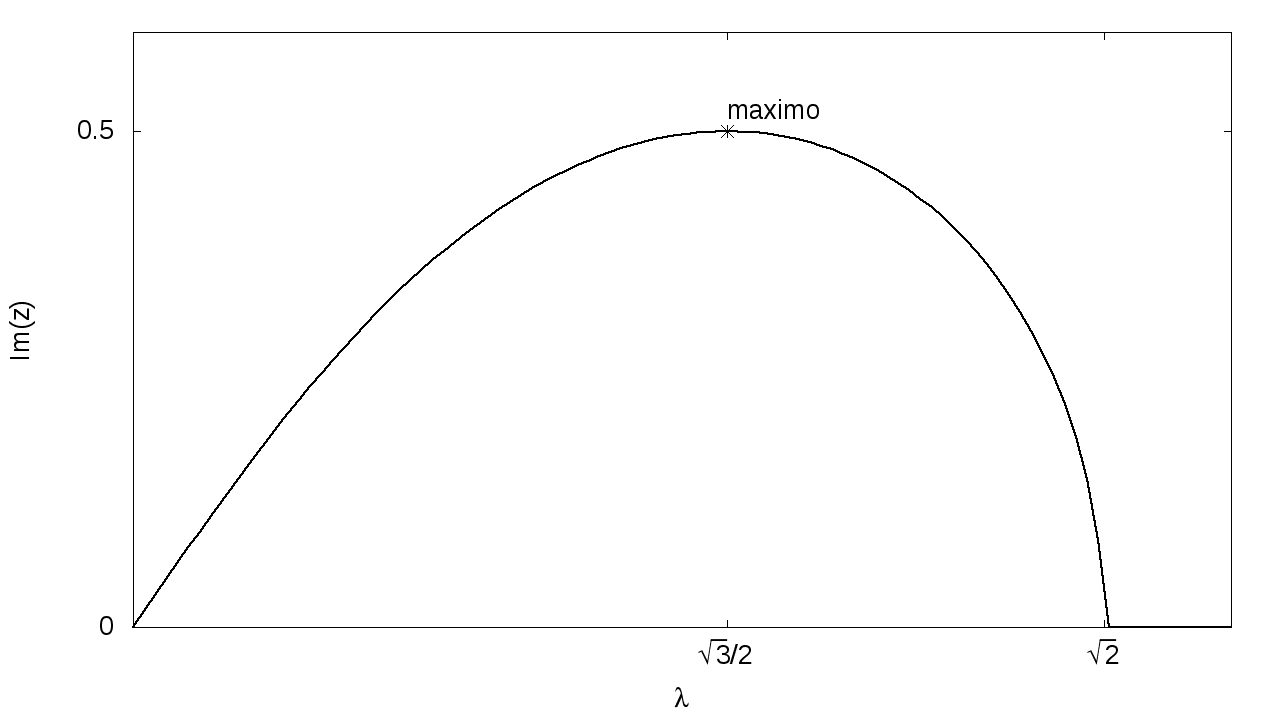
\includegraphics[height=0.3\paperheight]{grafica_misma_omega_contrarias.png}
\caption{Tasa de crecimiento para dos especies con misma $\omega_{p\sigma}^2$ pero con velocidades de signo contrario. Donde $\operatorname{Im}(z)_{max}=1/2$}
\label{fig:misma_omega_tasa_de_crecimiento}
\end{figure}
\subsection{Misma \texorpdfstring{$\boldsymbol{\omega_{p\sigma}}$}{w} con una especie incidente y la otra estacionaria.}
La relación de dispersión para este caso es muy similar a la ecuación \ref{dispersion_ep_adimensional}, el único cambio se da en recordar que una de las especies tiene velocidad cero, por lo tanto se tiene:
\begin{equation}
\label{eq:misma_omega_reposo}
1 = \frac{1}{z^2} + \frac{1}{(z-\lambda)^2}
\end{equation}
Al igual que el caso de dos especies con misma $\omega_{p\sigma}^2$ pero con velocidades de signo contrario, la raíz que nos es de interes es la raíz cuya parte imaginaria sea positiva, es decir en donde la perturbación crece exponencialmente con el tiempo. Para resolver la raíz se emplea el cambio de variable $z=x+\frac{\lambda}{2}$ lo que resulta en la siguiente expresión:
\begin{equation}
\label{eq:reducida_misma_reposo}
x^4 - \frac{1}{2}(4 + \lambda^2)x^2 + \frac{1}{16}\lambda^2 (\lambda^2 -8)=0
\end{equation}
La cuál es una ecuación bicuadrática de $x$ que permite entonces escribir:
\begin{equation}
\label{eq:bicuad_misma_reposo}
x^2 = \frac{1}{4}(4 + \lambda^2 \pm 4\sqrt{ \lambda^2 +1})
\end{equation}
De la cual se calcula la raíz para $x$ y se realiza el cambio de variable correspondiente para recuperar una solución en $z$.
\begin{equation}
\label{eq:solucion_misma_reposo}
z = \frac{1}{2}\left(\lambda + \sqrt{4 + \lambda ^2 - 4 \sqrt{1 + \lambda ^2}} \right)
\end{equation}
Los signos de la raíz se escogen para que la parte imaginaria de $z$ sea positiva. Para más detalle sobre la obtención de la raíz véase el apéndice \ref{Ap:raices}.
El siguiente paso es buscar el umbral en donde sucede la inestabilidad y para ello se estudia el lado derecho de la ecuación \ref{eq:misma_omega_reposo} y se observa que tiene dos singularidades $z=0,\lambda$. Aquí, el valor de $\lambda$ determinará el mínimo del lado derecho de \ref{eq:misma_omega_reposo} en el intervalo $(0,\lambda)$, al cual llamaremos $f(z,\lambda)$ por simplicidad. La figura \ref{fig:fz_reposo} ilustra el caso para una cierta $\lambda$, en donde se puede apreciar como el valor de $\lambda$ puede afectar el mínimo en el intervalo $(0,\lambda)$. El mínimo que nos interesa es el de valor $1$ pues ese índica cuando las raíces de ecuación \ref{eq:misma_omega_reposo} empiezan a ser imaginarias. Estrictamente hablando, cuando el mínimo es uno quiere decir que dos de sus raíces reales se vuelven una y es cuando el mínimo es mayor que uno que aparecen raíces imaginarias.
\begin{figure}
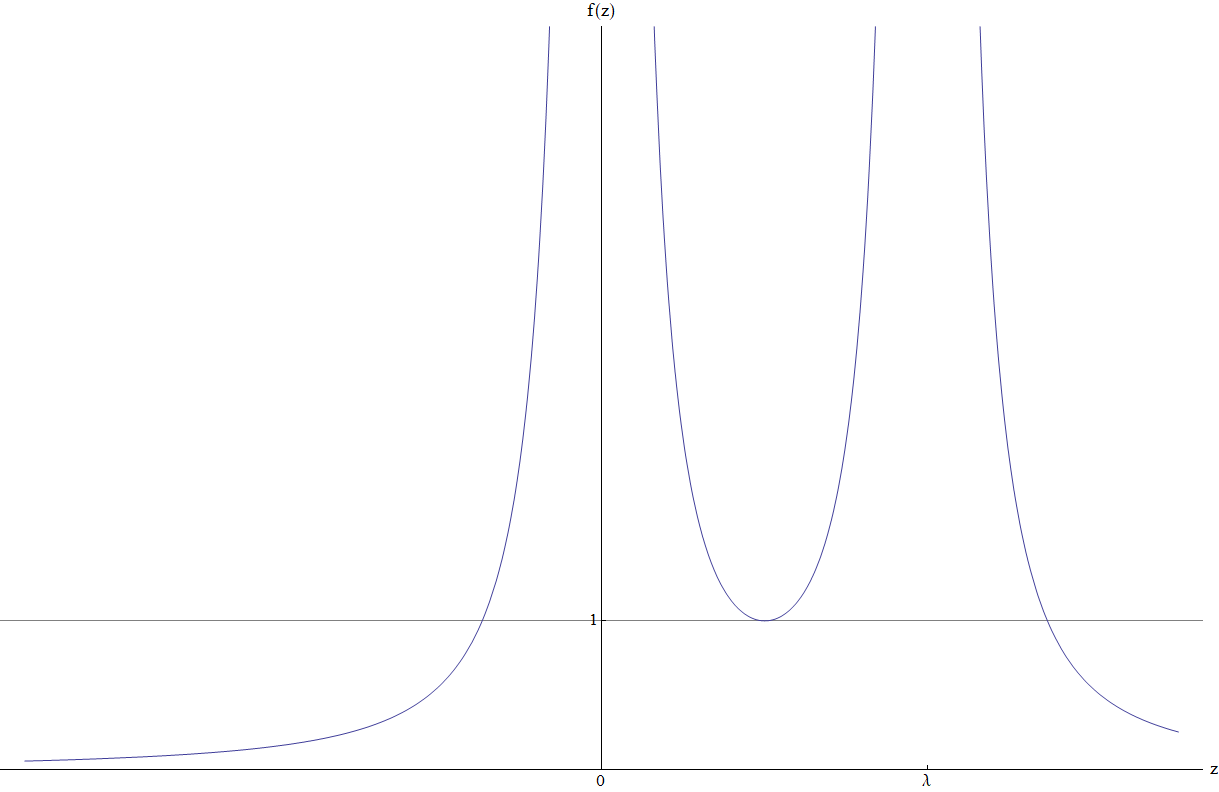
\includegraphics[height=0.3\paperheight]{f_z_reposo.png}
\caption{Gráfica del lado derecho de la ecuación \ref{eq:misma_omega_reposo} para un cierto valor de $\lambda$}
\label{fig:fz_reposo}
\end{figure}
Para encontrar ese umbral se busca entonces para que $\lambda$s el mínimo de $f(z,\lambda)$ es igual a uno. Se empieza entonces por minimizar.
\begin{equation}
\frac{1}{z^3} + \frac{1}{(z-\lambda)^3}=0
\end{equation}
El cual da $z=\lambda / 2$. Que al sustituir en \ref{eq:misma_omega_reposo} y resolver para $\lambda$ da $\lambda = \sqrt{8}$. Por lo que se tiene que el intervalo de inestabilidad es:
\begin{equation}
0 < \lambda < \sqrt{8}
\end{equation}
Para encontrar la máxima tasa de crecimiento se hace uso de que la ecuación \ref{eq:solucion_misma_reposo} representa un número complejo. Basta entonces buscar el máximo de la norma de dicho número. Se tiene entonces:
\begin{equation}
|z|^2 = \frac{1}{4}[\lambda^2 -4 - \lambda^2 + 4(1 + \lambda^2)^{1/2}]
\end{equation}
Donde al observar la ecuación \ref{eq:solucion_misma_reposo} vemos que los términos que le corresponden a la parte imaginaria son $-4 - \lambda^2 + 4(1 + \lambda^2)^{1/2}$. Es decir si $z=x +iy$:
\begin{equation}
y^2= -4 - \lambda^2 + 4(1 + \lambda^2)^{1/2}
\end{equation}
Que al maximizar con respécto de $\lambda$ da:
\begin{equation}
2\lambda -\lambda(1 + \lambda^2)^{1/2} =0
\end{equation}
Y al resolver para $\lambda$ se obtiene
\begin{equation}
\lambda = \sqrt{3}
\end{equation}
Estos valores se pueden apreciar en la figura \ref{fig:misma_omega_tasa_de_crecimiento} que grafica la parte imaginaria de $z$, es decir la correspondiente al crecimiento de la inestabilidad, contra $\lambda$. 
\begin{figure}[!h]
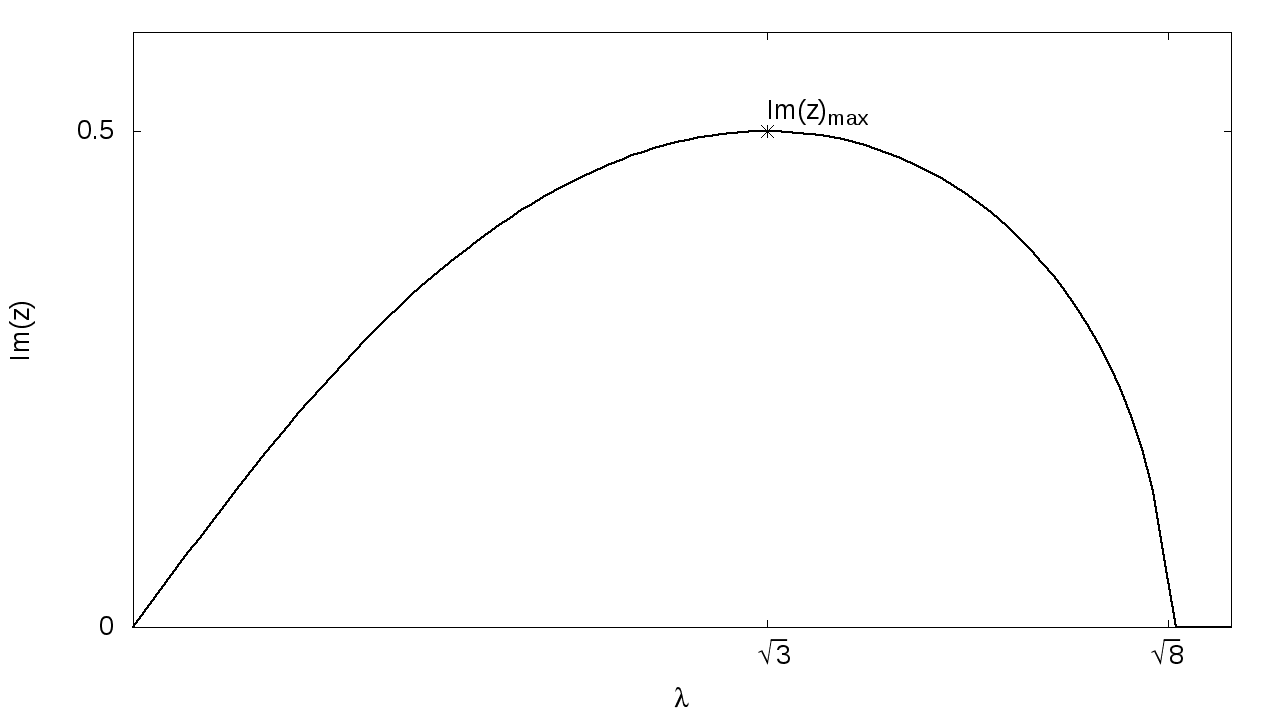
\includegraphics[height=0.3\paperheight]{grafica_misma_omega_reposo.png}
\caption{Tasa de crecimiento para dos especies con misma $\omega_{p\sigma}^2$ pero una de ellas estacionaria. Con $\operatorname{Im}(z)_{max}=1/2$}
\label{fig:misma_omega_reposo}
\end{figure}
Ahora bien regresando a variables físicas se tiene que el umbral de insetabilidad ocurre cuando
\begin{equation}
ku_0 < \sqrt{8} \omega_{p\sigma}
\end{equation}
Y la máxima tasa de crecimiento sucede cuando:
\begin{equation}
ku_0= \sqrt{3} \omega_{p\sigma}
\end{equation}
Y en cuyo caso se tiene
\begin{equation}
\omega = \frac{1}{2} (\sqrt{3} + i)\omega_{p\sigma}
\end{equation}
\subsection{Generalizando el caso para dos especies con la misma \texorpdfstring{$\boldsymbol{\omega_{p\sigma}}$}{w}}
Como se vió en el caso para mismas especies con velocidades opuestas, la relación de dispersión se reduce a una ecuación bicuadrática y de esa manera se encuentran las raíces de la ecuación cuártica. Ésta reducción es posible debido a la simetría del problema. Sin embargo, se tiene que al encontrar las raíces de la ecuación cuártica para el caso de una especie en reposo y otra especie incidente con cierta velocidad arbitraria, también se llega a una ecuación bicuadrática a pesar de no tener la misma simetría que el caso con dos velocidades opuestas. Dicha ecuación bicuadrática aparece como resultado de un cambio de variable $z=x+\lambda /2$, para más detalle véase el apéndice \ref{Ap:raices}. Esto podría sugerir que para dos especies con la misma $\omega_{p\sigma}$ su relación de dispersión siempre se puede reducir a una ecuación bicuadrática con el cambio de variable apropiado. Independientemente de la velocidad que lleve cada especie.\\
Una manera de hacer esto sería partir del caso general y aplicar el cambio de variable sugerido en el apéndice \ref{Ap:raices} para comprobar que se obtiene una ecuación bicuadrática. Sin embargo, otra manera de proceder es partir del caso de una especie en reposo y por medio de un cambio de variable recuperar el caso general.
Se empieza entonces por la relación de dispersión del caso de una especie estacionaria y otra incidente, ambas con la misma $\omega_{p\sigma}$, es decir la ecuación \ref{eq:misma_omega_reposo}.
\begin{equation*}
1 = \frac{1}{z^2} + \frac{1}{(z-\lambda)^2}
\end{equation*}
Si se graficara el lado derecho de la ecuación en función de $z$, véase la figura \ref{fig:fz_reposo}, se observa que los valores de $z$ para los que aparecen raíces complejas se encuentran en el intervalo $(0, \lambda)$. Por otro lado, se puede ver este caso como uno con dos velocidades en donde una de las velocidades resulta ser cero y por lo tanto su $\lambda$ asociada es cero. Se tiene entonces que la distancia entre las dos $\lambda$s es precisamente $\lambda$.\\
Una manera más simple de ver esto es considerando también los otros valores posibles para cada una de las $\lambda$s, recordando que son reales, estos casos son ilustrados en la figura \ref{fig:valores_lambda}.
\begin{figure}[h]
\centering
 \begin{subfigure}[b]{0.4\textwidth}
 	 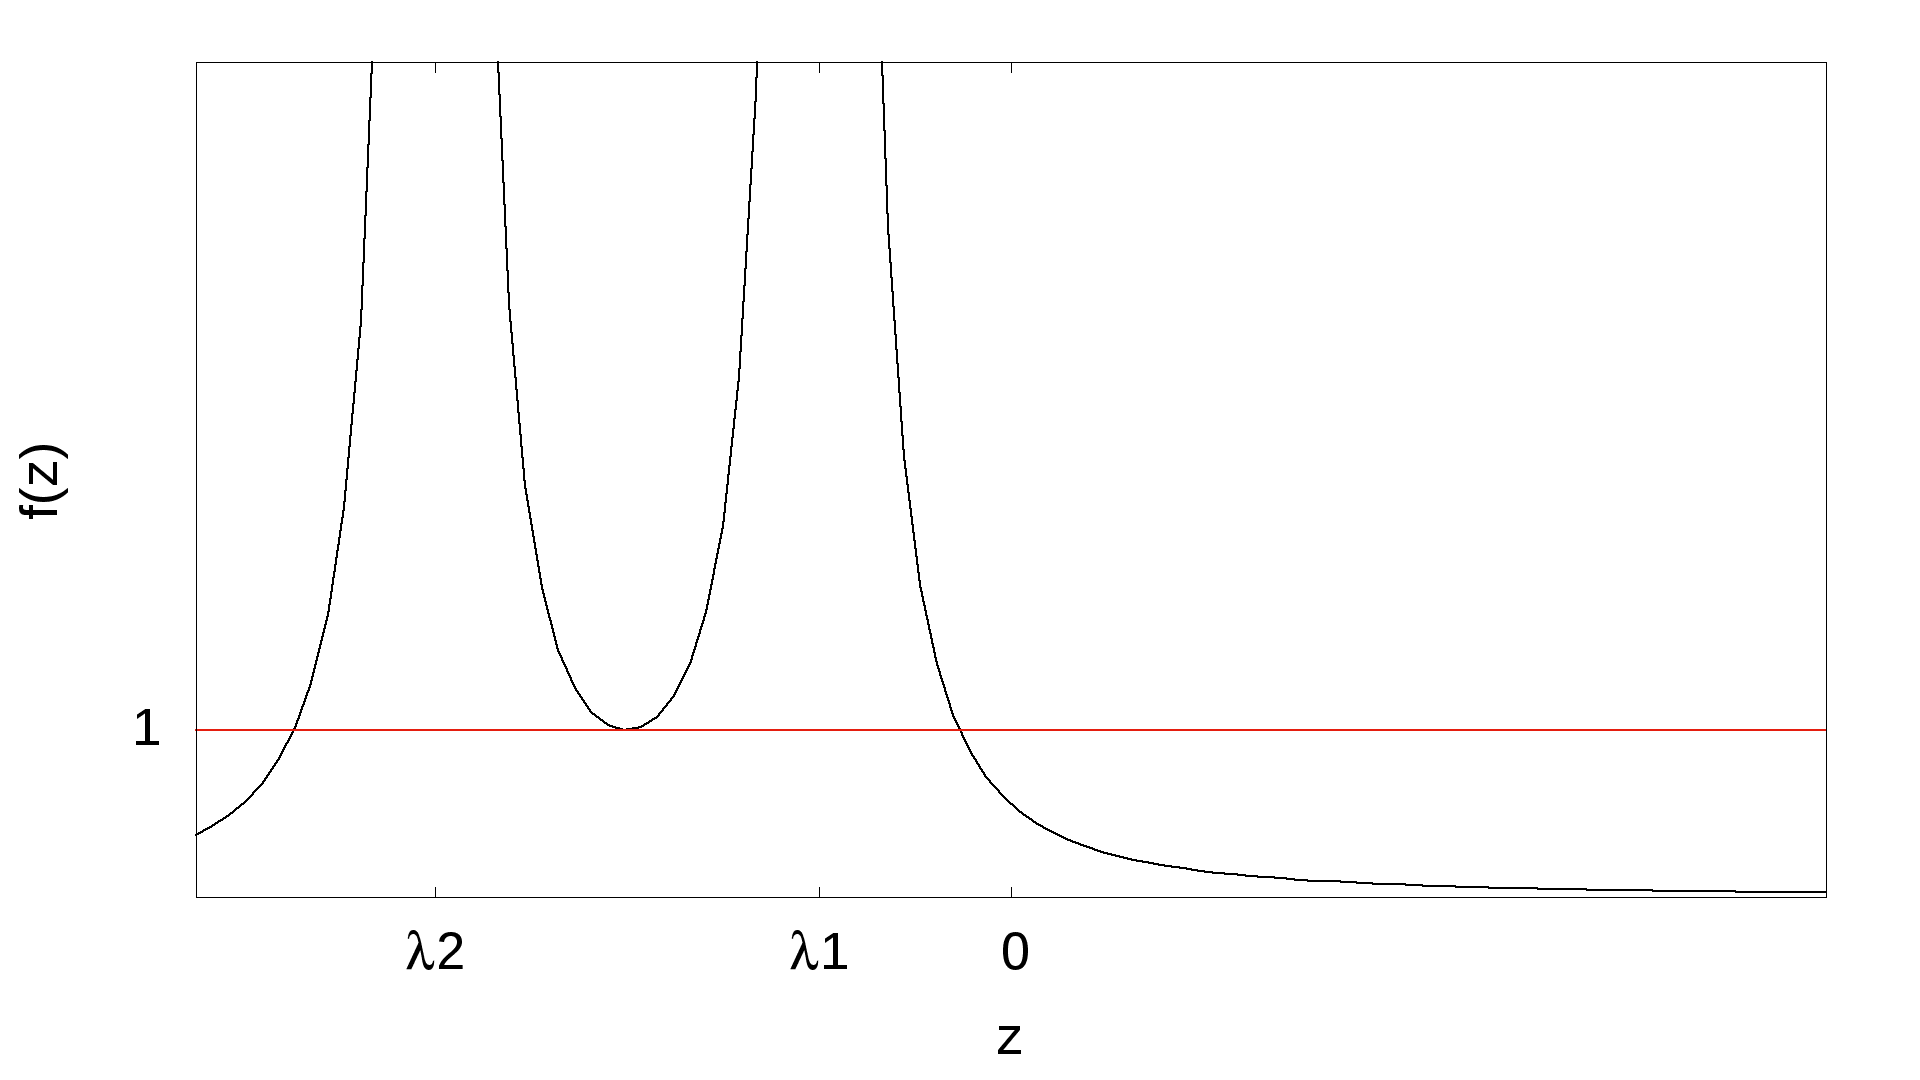
\includegraphics[width=\textwidth]{grafica_lambdas_negativas.png}
 	 \caption{}
 	 \label{fig:lamdas_negativas}
 \end{subfigure}
 
 \begin{subfigure}[b]{0.4\textwidth}
 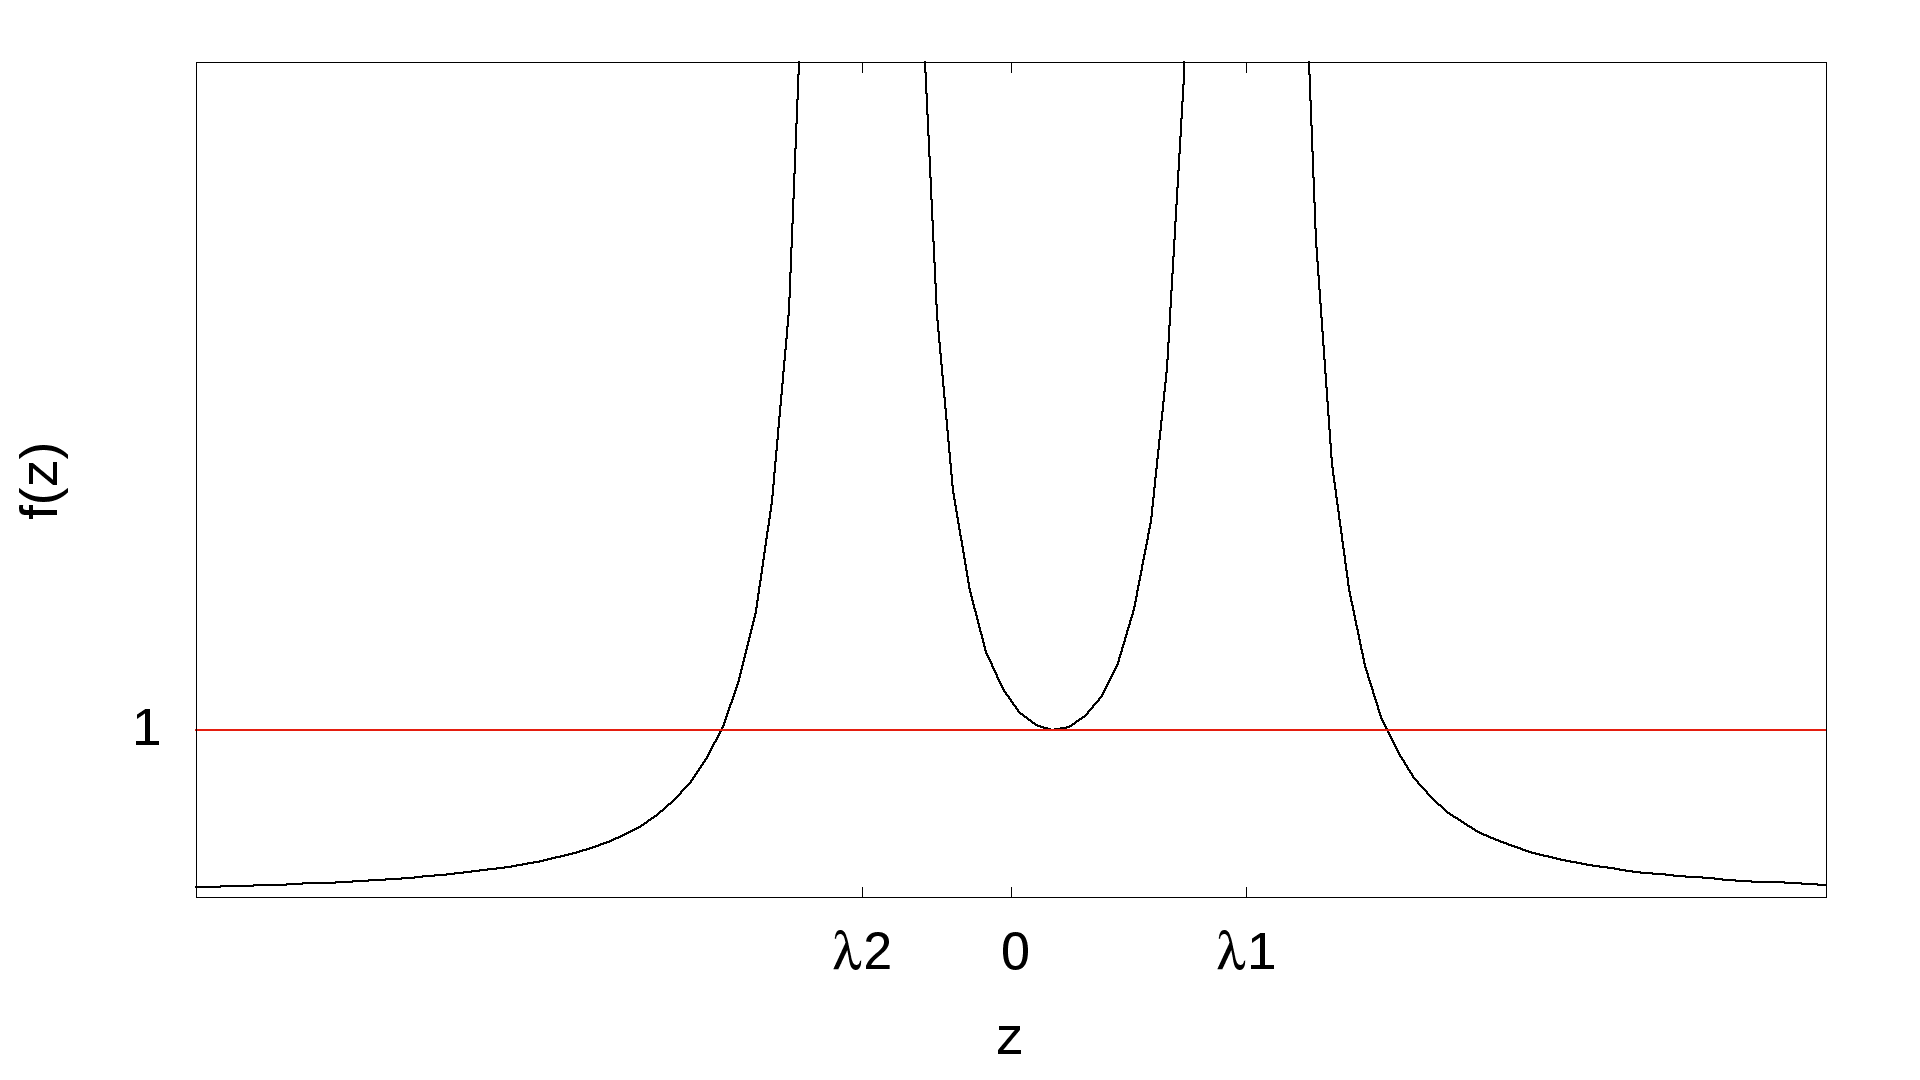
\includegraphics[width=\textwidth]{grafica_lambdas_alternadas.png}
 \caption{}
 \label{fig:lamdas_alternadas}
 \end{subfigure}
 ~
  \begin{subfigure}[b]{0.4\textwidth}
 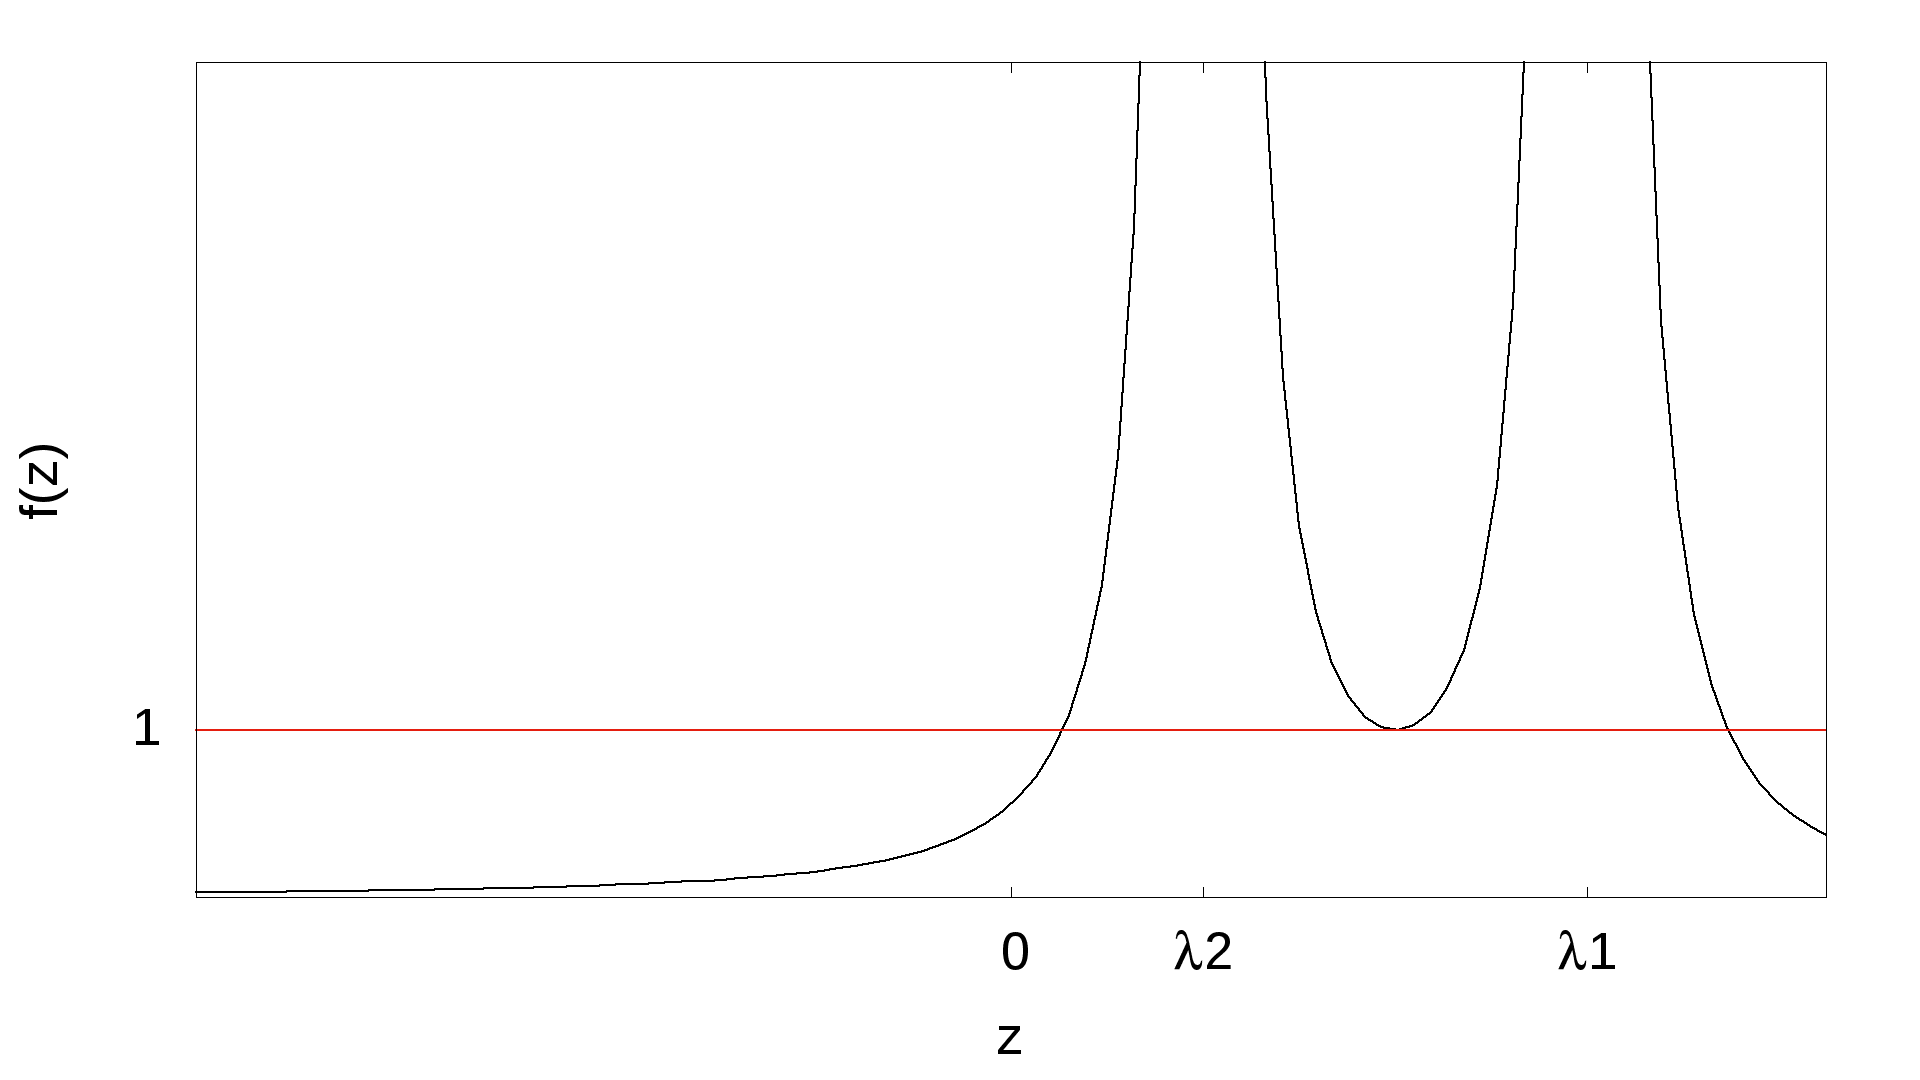
\includegraphics[width=\textwidth]{grafica_lambdas_positivas.png}
  \caption{}
 \label{fig:lamdas_positivas}
 \end{subfigure}
 \caption{Representaciones de los distintos valores que $\lambda_1$ y $\lambda_2$ pueden tomar. Siendo estos cuando ambas son negativas, cuando una es negativa y la otra es positiva y el caso donde ambas son positivas.}\label{fig:valores_lambda}
\end{figure}
Se tiene entonces que se puede definir una distancia $\lambda$ entre $\lambda_1$ y $\lambda_2$ de la forma $\lambda = \lambda_1 - \lambda_2$. La cual permite ver que la ecuación \ref{eq:misma_omega_reposo} es un caso donde $\lambda_2 =0$ y por lo tanto $\lambda_1 = \lambda$. No está de más entonces suponer que si se tiene $\lambda$ constante se puedan recuperar los casos de velocidades opuestas y el de velocidades arbitrarias a partir de una traslación del caso en reposo.\\
Dicha traslación se propone como el cambio de variable $z=z'-\lambda_2$ y recordando que se está tomando $\lambda= \lambda_1 - \lambda_2$ se llega a:
\begin{equation}
\label{eq:misma_omega_general}
1 = \frac{1}{(z'-\lambda_2)^2} + \frac{1}{(z'-\lambda_1)^2}
\end{equation}
Que es el caso general para dos especies con misma $\omega_{p\sigma}$ y velocidades arbitrarias. Lo que la ecuación \ref{eq:misma_omega_general} expone es que el caso de dos velocidades de signo contrario se puede recuperar del caso en reposo ya se haciendo $\lambda_2 = -\lambda_1$ en \ref{eq:misma_omega_general} o realizando el cambio de variable $z=z' +\lambda_1$ y $\lambda= 2\lambda_1$ en \ref{eq:misma_omega_reposo}. Cualquiera de los dos métodos da la expresión:
\begin{equation}
\label{eq:misma_omega_opuestas_cambio}
1 = \frac{1}{(z'+\lambda_1)^2} + \frac{1}{(z'-\lambda_1)^2}
\end{equation}
La cual sabemos se reduce a una ecuación bicuadrática.\\
Del caso de una especie en reposo se tenía que el umbral era:
\begin{equation}
0<\lambda<\sqrt{8}
\end{equation}
Que pasandolo al caso general se tiene:
\begin{equation}
0<\lambda_1 - \lambda_2 <\sqrt{8}
\end{equation}
Por otro lado la máxima tasa de crecmiento sucedía cuando
\begin{equation}
\lambda=\sqrt{3}
\end{equation}
Que resulta ser 
\begin{equation}
\lambda_1 - \lambda_2 = \sqrt{3}
\end{equation}
%\subsection*{Caso con $\omega_{p\sigma}$ diferentes y una especie estacionaria.}
%
\subsection{Plasma estacionario y plasma incidente}
Este caso consiste en un plasma compuesto por dos especies que se mueven a una velocidad $\overrightarrow{\textbf{u}}_{\sigma 0}$ incidiendo con un plasma estacionario compuesto por las mismas especies. Se trata entonces de un caso de cuatro especies. Cuya relación de dispersión normalizada es de la forma:
\begin{equation}
\label{eq:disp_d-d}
\frac{\epsilon_1}{z^2}+\frac{1}{z^2}+\frac{\epsilon_1}{(z-\lambda)^2}+\frac{1}{(z-\lambda)^2}=1
\end{equation}
Donde $\epsilon_1 = \omega_{p1}/ \omega_{pe}$. Para encontrar el umbral de inestabilidad se realiza el mismo procedimiento de los casos anteriores. Se minimiza la ecuación \ref{eq:disp_d-d} y se resuelve para obtener $z$ en términos de $\lambda$. Que resulta ser $z=\lambda /2$.
\begin{equation}
\frac{\epsilon_1}{z^3}+\frac{1}{z^3}+\frac{\epsilon_1}{(z-\lambda)^3}+\frac{1}{(z-\lambda)^3}=0
\end{equation}
Si se sustituye en \ref{eq:disp_d-d} y se resuelve para $\lambda$ se encuentra entonces que:
\begin{equation}
0 < \lambda < \sqrt{8(1+\epsilon)}
\end{equation}
Para encontrar la máxima tasa de crecimiento se empieza por buscar la raíz del lado derecho de \ref{eq:disp_d-d} que tenga parte imaginaria positiva. Dicha raíz resulta ser:
\begin{equation}
\label{eq:raiz_d-d}
z =\frac{1}{2}\left(\lambda + \sqrt{4 + 4\epsilon + \lambda ^2 -4\sqrt{1+2\epsilon + \epsilon^2+ \lambda^2 + \epsilon \lambda ^2}} \right)
\end{equation}
La cual también se multiplica por su conjugado para así obtener el cuadrado de su componente imaginaria.
\begin{equation}
y^2 = -\left(4 + 4\epsilon + \lambda ^2 -4\sqrt{1+2\epsilon + \epsilon^2+ \lambda^2 + \epsilon \lambda ^2}\right)
\end{equation}
El cual se maximiza con respecto a $\lambda$ y al resolver da $\lambda = \sqrt{3(1 + \epsilon)}$. La cual se sustituye en la ecuación \ref{eq:disp_d-d} para dar:
\begin{equation}
\label{eq:z-max-d-d}
z_{max} = \frac{1}{2}\left(\sqrt{3(1+\epsilon)} + i \sqrt{(1+\epsilon)} \right)
\end{equation}
%Al tratarse de el caso de deuterio, se tiene que $\epsilon = 2.72 \times 10^{-4}$. Que al sustituir en la ecuación \ref{eq:z-max-d-d} da:
%\begin{equation}
%z=0.86614 + 0.50007i
%\end{equation}
%Entonces, el umbral de inestabilidad resulta ser:
%\begin{equation}
%0 < \lambda < 2.82881
%\end{equation}
%Y la máxima tasa de crecimiento sucede cuando $\lambda = 1.73229$.
%Esto se traduce como:
%\begin{equation}
%ku_0 < 2.82881 \omega_{pe}
%\end{equation}
%Para el umbral de inestabilidad.
%\begin{equation}
%ku_0 = 1.73229 \omega_{pe}
%\end{equation}
%Para el valor al cual aparece la máxima tasa de crecimiento.
%\begin{equation}
%\omega = (0.86614 + 0.50007i)\omega_{pe}
%\end{equation}
%Y finalmente la expresión para la frecuencia cuando ésta ocurre. 
La figura \ref{fig:d-d} muestra el comportamiento de la parte imaginaria de $z$ para el caso que se acaba de estudiar.
\begin{figure}
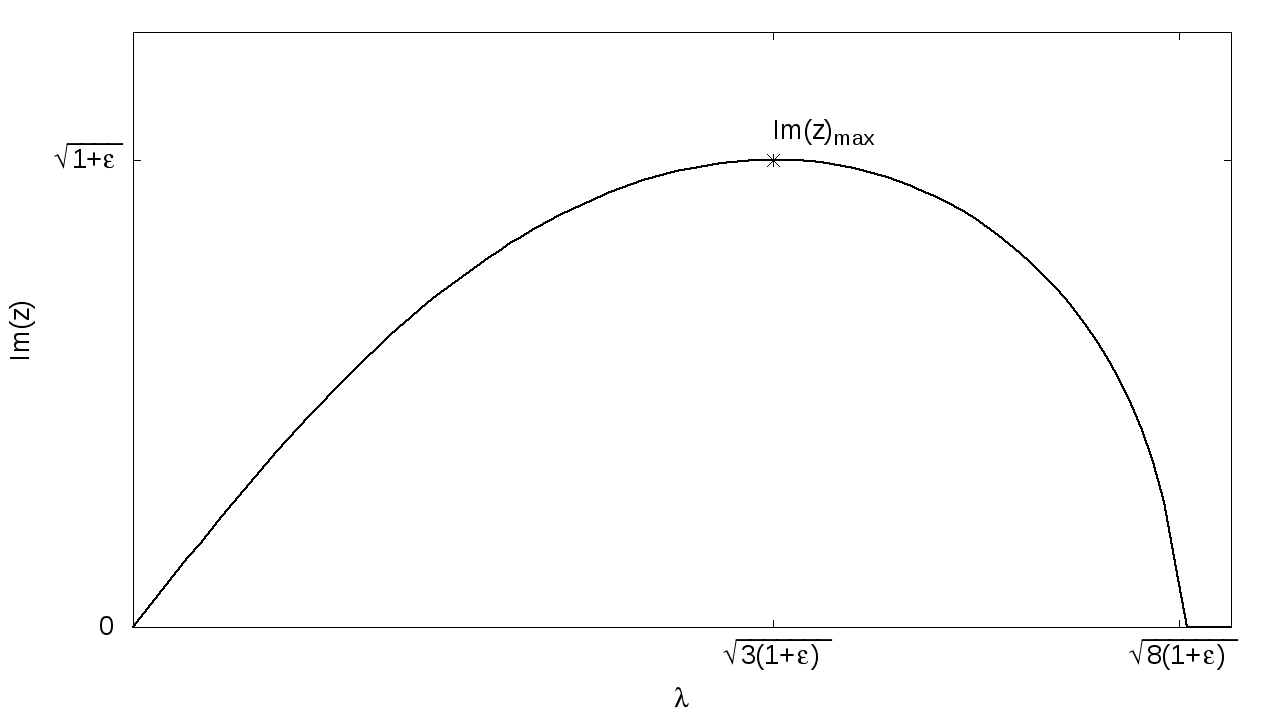
\includegraphics[height=0.3\paperheight]{grafica-d-d-reposo}
\caption{$Im(z)$ en función de $\lambda$, para el caso de un haz de dos especies incidiendo con un plasma estacionario de dos especies. Con $\operatorname{Im}(z)_{max}=\frac{1}{2}\sqrt{(1+\epsilon)}$}
\label{fig:d-d}
\end{figure}
\subsection{Iones estacionarios y electrones incidentes}
La relación de dispersión para este caso es la siguiente:
\begin{equation}
\label{eq:disp_ion_electron}
\frac{\epsilon}{z^2}+\frac{1}{(z-\lambda)^2}=1
\end{equation}
Donde $z$ y $\lambda$ son las constantes normalizadas de los casos anteriores, mientras que $\epsilon = m_e/m_i$.
Siguiendo el proceso que se ha estado haciendo, lo primero que se busca es el umbral de inestabilidad. Es decir para que valores de $\lambda$ dos raíces reales colapsan a una sola o aparecen raíces complejas. Como ya se había mencionado, esto sucede cuando el mínimo del lado izquierdo de la ecuación \ref{eq:disp_ion_electron} es mayor o igual a la unidad. Si se toma al lado izqueirdo de \ref{eq:disp_ion_electron} como una función $f(z,\lambda)$ y se minimiza se llega a una expresión:
\begin{equation}
\frac{\epsilon}{z^3}+\frac{1}{(z-\lambda)^3}=0
\end{equation}
De donde se busca tener exponentes positivos para $z$ por lo que se manipula para obtener:
\begin{equation}
\frac{z^3}{\epsilon}=-(z-\lambda)^3
\end{equation}
De donde se pueden obtener raíces cúbicas de cada término:
\begin{equation}
\frac{z}{\epsilon ^{1/3}}=-(z-\lambda)
\end{equation}
De la cual se despeja $z$
\begin{equation}
z_{min}=\frac{\epsilon ^{1/3}\lambda}{(1- \epsilon^{1/3})}
\end{equation}
Que es el valor que la variable $z$ debe tener para que el mínimo sea uno. Está $z_{min}$ se puede substituir en la relación de dispersión para llegar al valor de $\lambda$ que buscamos:
\begin{equation}
1=f(z_{min},\lambda)=\frac{(1+\epsilon^{1/3})^3}{\lambda^2}
\end{equation}
Entonces, para que el mímimo sea mayor o igual a uno el valor de $\lambda$ debe ser:
\begin{equation}
\label{eq:umbral_ion_electron}
\lambda \geq (1+\epsilon^{1/3})^{3/2}
\end{equation}
El cual es nuestro umbral de inestabilidad.
El siguiente paso es entonces buscar una raíz para $z$ en la expresión \ref{eq:disp_ion_electron} que describa el crecimiento de una inestabilidad. Sin embargo, a diferencia de los casos anteriores la ecuación \ref{eq:disp_ion_electron} no se reduce a una ecuación bicuadrática al hacer el cambio de variable y por ello el procedimiento para encontrar la raíz es más laborioso. A continuación se muestra a grandes razgos el cálculo de la raíz, el procedimiento se encuentra con mayor detalle en el apéndice \ref{Ap:raices}.\\
Al expandir la ecuación \ref{eq:disp_ion_electron} y realizando el cambio de vairable $z=x+\frac{\lambda}{2}$ se llega a:
\begin{equation}
x^4 + (-\frac{\lambda^2}{2} -\epsilon -1)x^2 + (\epsilon \lambda - \lambda)x + \frac{\lambda^4}{16}-\frac{\epsilon \lambda^2}{4}-\frac{\lambda^2}{4}=0
\end{equation}
De cuyos coeficientes se construye una expresión para el término auxiliar $\alpha_0$ que es de la forma:
\begin{multline}
\alpha_0 = \frac{1}{3}\left(\frac{\lambda^2}{2} + \epsilon + 1 \right)\\
+ \left(\frac{1}{216}\lbrace-\epsilon^3+3\epsilon^2(\lambda^2-1)-
3\epsilon(\lambda^4 +16\lambda^2 +1)+ (\lambda^2 -1)^3\rbrace \right. \\
\left. +\frac{\lambda}{12\sqrt{3}}\lbrace\epsilon [\epsilon^3-3\epsilon^2(\lambda^2 -1)+3\epsilon(\lambda^4 + 7\lambda^2 +1)- (\lambda^2-1)^3]\rbrace^{1/2} \vphantom{\frac{1}{216}}\right)^{1/3}\\
+ \left(\frac{1}{216}\lbrace-\epsilon^3+3\epsilon^2(\lambda^2-1)-
3\epsilon(\lambda^4 +16\lambda^2 +1)+ (\lambda^2 -1)^3\rbrace \right. \\
\left. -\frac{\lambda}{12\sqrt{3}}\lbrace\epsilon [\epsilon^3-3\epsilon^2(\lambda^2 -1)+3\epsilon(\lambda^4 + 7\lambda^2 +1)- (\lambda^2-1)^3]\rbrace^{1/2} \vphantom{\frac{1}{216}}\right)^{1/3}
\end{multline}
Una vez obtenido $\alpha_0$ se puede encontrar entonces una raíz para $x$ cuya parte imaginaria sea postiva y al volver a realizar un cambio de variable se recupera la raíz para $z$.
\begin{equation}
z= \frac{1}{2} \left( \lambda + \sqrt{2\alpha_0} + \sqrt{2\alpha_0 -4 \left(-\frac{1}{2}(\frac{\lambda^2}{2}+\epsilon+1)+\alpha_0 +\frac{\epsilon \lambda - \lambda}{2\sqrt{2\alpha_0}}\right)}\right)
\end{equation}
\section{Transferencia de energía}
Se empieza con proponer un potencial de onda unidimensional.
\begin{equation}
\label{eq:potencial_sinosoidal}
\Phi(x,t) = \Phi_0 cos(kx-\omega t)
\end{equation}
Esto corresponde a una partícula sobre la cual está actuando una onda que se mueve en la dirección positiva de x con velocidad de fase $\omega /k$. Si se asume que no hay campo magnético, la ecuación de movimento es de la forma:
\begin{equation}
\label{eq:mov_sen_particula}
\frac{dv}{dt}=\frac{qk\Phi_0}{m}sen(kx-\omega t)
\end{equation}
Cuyas condiciones iniciales para un tiempo $t=0$ son $x_0$ y $v_0$. En este caso la $v_0$ se refiere a la velocidad de inyección de la partícula.\\
Se tiene que en el sistema de referencia de la onda, la energía es una constante de movimiento ya que el hamiltoniano es independiente del tiempo en el sistema de referencia de la onda por lo que resultaria conveniente trabajar sobre este. Para ello se introduce la variable $\psi= kx - \omega t$, que viene siendo la fase de la onda en la posición de la partícula. La razón para introducir esta variable es debido a que al hacer $\psi$ la variable dependiente es equivalente a realizar una transformación al sistema de la onda. Por último, resulta más conveniente trabajar con la variable de fase modificada $\theta = kx -\omega t -\pi$, pues evitara lidiar con algunos signos negativos. De esta manera la primera y segunda derivadas de $\theta$ son:
\begin{equation}
\label{eq:deriv_theta}
\frac{d\theta}{dt}=kv -\omega
\end{equation}
\begin{equation}
\label{eq:segunda_deriv_theta}
\frac{d^2\theta}{dt^2}=k \frac{dv}{dt}
\end{equation}
Sustituyendo entonces la ecuación \ref{eq:mov_sen_particula} en la segunda derivada de $\theta$ se obtiene:
\begin{equation}
\label{eq:seg_deriv_theta_sustitucion}
\frac{d^2\theta}{dt^2}=\frac{qk^2\Phi_0}{m}sen(\theta + \pi)
\end{equation}
O bien:
\begin{equation}
\label{eq:seg_deriv_th_simple}
\frac{d^2\theta}{dt^2}+\omega_b^2 sen(\theta)=0
\end{equation}
Donde se ha definido a $\omega_b^2 = qk^2\Phi_0/m$ como la frecuencia de rebote. Si además se define una variable adimensional $\tau = \omega_b t$ como el tiempo normalizado de rebote, la ecuación \ref{eq:seg_deriv_th_simple} se puede escribir como:
\begin{equation}
\label{eq:mov_theta_tau}
\frac{d^2\theta}{d\tau^2}+sen(\theta)=0
\end{equation}
Al estar en el marco de referencia de la onda sería conveniente encontrar una expresión para el hecho de que la energía es una constante de movimiento en el sistema de la onda. Dicha expresión se puede encontrar si se multiplica la ecuación \ref{eq:mov_theta_tau} por el factor integrante $2d\theta/d\tau$.
\begin{equation}
2\frac{d\theta}{d\tau}\frac{d}{d\tau}\left(\frac{d\theta}{d\tau}\right) + 2\frac{d\theta}{d\tau}sen(\theta)=0
\end{equation}
La cual se puede escribir como
\begin{equation}
\label{eq:energia_constante_1}
\frac{d}{d\tau}\left[\left(\frac{d\theta}{d\tau}\right)^2 -2cos(\theta)\right]=0
\end{equation}
Que al integrar da:
\begin{equation}
\label{eq:energia_const_onda}
\left(\frac{d\theta}{d\tau}\right)^2 -2cos(\theta)=\eta=cte
\end{equation}
La ecuación \ref{eq:energia_const_onda} es la expresión para la conservación de la energía que se estaba buscando salvo un factor constante.\\
El término $\eta$ se determina a partir de las condiciones iniciales del sistema las cuales son: la velocidad de inyección en el sistema de referencia de la onda
\begin{equation}
\label{eq:wave_frame_injection_velocity}
\left(\frac{d\theta}{d\tau}\right)_{\tau =0}=\frac{1}{\omega_b}\left(\frac{d\theta}{dt}\right)_{t=0}=\frac{1}{\omega_b}(kv_0-\omega)=\alpha
\end{equation}
Y la fase de inyección en el sistema de referencia de la onda
\begin{equation}
\label{eq:wave_frame_injection_phase}
\theta_{\tau=0}=kx_0-\pi=\theta_0
\end{equation}
Por lo que $\eta$ se puede expresar como
\begin{equation}
\label{eq:expresion_eta_wave_frame}
\eta = \alpha^2 -2cos(\theta_0)
\end{equation}
Como ya se habia mencionado, $\eta$,$\alpha^2$ y $-2cos(\theta_0)$ son términos para la energía total, cinética y potencial respectivamente salvo un factor constante en el sistema de la onda.\\
Al ser términos referentes a la energía, $\alpha^2$ y $-2cos(\theta_0)$, o mejor dicho la relación entre esos términos, dan información acerca del comportamiento de la partícula sujeta al potencial que se definió al principio. En particular se hablará se cuando una partícula está atrapada en alguna región del potencial, lo cual corresponderá al caso cuando la energía cinética de la partícula es menor que la energía potencial, y el caso en el que la partícula no se encuentra atrapada por el potencial, es decir que su energía cinética es mayor que la energía potencial.\\
De la ecuación \ref{eq:expresion_eta_wave_frame} se tiene entonces
\begin{itemize}
\item Si $\alpha^2 < |2cos(\theta_0)| \Rightarrow -2<\eta<2$ y se habla de una partícula atrapada.
\item Si $\alpha^2 > |2cos(\theta_0)| \Rightarrow \eta>2$ y se habla de una partícula no atrapada y que se me mueve continuamente en una dirección pero cuya velocidad se verá afectada dependiendo de en que parte del potencial se encuentre.
\end{itemize}
Por el momento se considera solamente el caso donde la energía cinética de la partícula es mucho mayor que la energía potencial, es decir cuando $\alpha^2 \gg 2$ y se buscará determinar la manera en la que estas partículas no atrapadas intercambian energía con la onda. Cabe mencionar, que dadas las definiciones de $\alpha$, ecuación \ref{eq:wave_frame_injection_velocity}, y de $\omega_b$, se tiene $\alpha^2 \sim \Phi_0^{-1}$ por lo que un valor de $\alpha^2 \gg 2$ implica un valor para $\Phi_0 \ll 2$. Donde $\Phi_0$ viene siendo la amplitud de la onda. Por lo que el caso que se va a estudiar corresponde a ondas con amplitudes pequeñas.\\
Para poder determinar la energía transferida entre la onda y la partícula se debe poder expresar la energía cinética de la partícula en términos de cantidades del sistema de la onda. Para ello se utiliza la ecuación \ref{eq:deriv_theta} y la definición de $\tau$ para primero despejar la velocidad en el sistema del laboratorio y luego expresarla en términos de cantidades encontradas en el sistema de la onda.
\begin{equation}
\label{eq:velocidad_lab_transferencia}
v =\frac{1}{k}\left(\omega +\frac{d\theta}{dt}\right)= \frac{\omega_b}{k}\left(\frac{\omega}{\omega_b} +\frac{d\theta}{d\tau}\right)
\end{equation}
Entonces, la energía cinética se puede expresar como
\begin{equation}
\label{eq:energia_cintetica_1}
W = \frac{1}{2}mv^2=\frac{m\omega_b^2}{2k^2}\left[\frac{\omega^2}{\omega_b^2}+2\frac{\omega}{\omega_b}\frac{d\theta}{d\tau}+\left(\frac{d\theta}{d\tau}\right)^2\right]
\end{equation}
El término cuadrático de la derivada se puede sustitur utilizando la ecuación \ref{eq:energia_const_onda} y entonces la energía cinética de la partícula está dada por:
\begin{equation}
\label{eq:energia_cinetica_2}
W = \frac{m\omega_b^2}{2k^2}\left[\frac{\omega^2}{\omega_b^2}+2\frac{\omega}{\omega_b}\frac{d\theta}{d\tau}+\eta+ 2cos(\theta)\right]
\end{equation}
El siguiente paso es entonces determinar como va variando $W$ con respecto del tiempo
\begin{equation}
\label{eq:derivada_temp_W_1}
\frac{dW}{dt}=\frac{m\omega_b^3}{k^2}\left[\frac{\omega}{\omega_b}\frac{d^2\theta}{d\tau^2}-2\frac{d\theta}{d\tau}sen(\theta)\right]=-\frac{m\omega_b^3}{k^2}sen(\theta)\left[\frac{\omega}{\omega_b}+\frac{d\theta}{d\tau}\right]
\end{equation}
Donde se ha vuelto a utlizar la definición de $\tau$, junto con la regla de la cadena y la ecuación \ref{eq:mov_theta_tau}.\\
Lo que prosigue es encontrar la dependencia temporal de los términos $sen(\theta)$ y $d\theta /d\tau$. Se empieza entonces por despejar la derivada de la ecuación \ref{eq:energia_const_onda} y sustituyendo \ref{eq:expresion_eta_wave_frame} en ella.
\begin{equation}
\label{eq:despeje_deriv_theta_tau}
\frac{d\theta}{d\tau}=\pm \sqrt{\eta + 2cos(\theta)}=\pm \sqrt{\alpha^2+2cos(\theta)-2cos(\theta_0)}=\alpha \left(1 + \frac{2(cos(\theta)-cos(\theta_0))}{\alpha^2}\right)^{1/2}
\end{equation}
Donde al usar el hecho de que se está estudiando el caso de amplitudes pequeñas $\alpha \gg 1$ se llega a la aproximación.
\begin{equation}
\label{eq:aproximation_deriv_theta_tau}
\frac{d\theta}{d\tau}\simeq \alpha + \frac{cos(\theta)-cos(\theta_0)}{\alpha}
\end{equation}
De la ecuación \ref{eq:aproximation_deriv_theta_tau} el primer término corresponde a la velocidad de la partícula cuando no está sufriendo perturbación alguna, mientras que el segundo término es la perturbación debida a una onda de amplitud pequeña.\\
Lo que prosigue es hacer una aproximación mediante la cual se pueda encontrar una expresión para $\theta(\tau)$. Se empieza por el orden más bajo donde la velocidad de la partícula es entonces:
\begin{equation}
\label{eq:deriv_theta_tau_approximation_lowest}
\frac{d\theta}{d\tau}=\alpha
\end{equation}
Sustituyendo esta velocidad en la ecuación \ref{eq:derivada_temp_W_1} se obtiene:
\begin{equation}
\label{eq:deriv_w_approximation_lowest}
\frac{dW}{dt}=-\frac{m\omega_b^3}{k^2}sen(\theta)\left[\frac{\omega}{\omega_b}+\frac{kv_0-\omega}{\omega_b}\right]=-\frac{m\omega_b^2v_0}{k}sen(\theta)
\end{equation}
Integrando la ecuación \ref{eq:deriv_theta_tau_approximation_lowest} se obtiene:
\begin{equation}
\label{eq:theta_tau_lowest_approximation}
\theta(\tau)=\theta_0 +\alpha \tau
\end{equation}
La ecuación \ref{eq:theta_tau_lowest_approximation} es la solución para la órbita no perturbada. Si se sustituye en la ecuación \ref{eq:aproximation_deriv_theta_tau} se tiene entonces
\begin{equation}
\label{eq:sust_deriv_theta_tau_approximation}
\frac{d\theta}{d\tau}=\alpha \frac{cos(\theta_0+\alpha \tau)-cos(\theta_0)}{\alpha}
\end{equation}
Que al integrarse da la solución no perturbada más la corrección de fase
\begin{equation}
\label{eq:theta_tau_first_correction}
\theta(\tau)=\theta_0 +\alpha\tau +\frac{sen(\theta_0 + \alpha\tau)-sen(\theta_0)}{\alpha^2}-\frac{\tau}{\alpha}cos(\theta_0)
\end{equation}
Se puede definir entonces un término, dígase $\Delta$, como la corrección de fase de la órbita perturbada de la siguiente manera.
\begin{equation}
\label{eq:perturbed_orbit_correction_phase}
\Delta (\tau)=\frac{sen(\theta_0 + \alpha\tau)-sen(\theta_0)}{\alpha^2}-\frac{\tau}{\alpha}cos(\theta_0)
\end{equation}
De está manera se puede escribir una expresión de la dependencia temporal de $sen(\theta)$.
\begin{equation}
\label{eq:sen_approximation_with_correction}
sen(\theta(\tau))=sen[\theta_0 + \alpha\tau + \Delta(\tau)]
\end{equation}
Ahora bien, si se hace la restricción para el caso donde los tiempos son lo suficientemente pequeños tales que $\tau \ll |\alpha|$, entonces la corrección de fase $\Delta(\tau)$ será pequeña. La restricción a este caso corresponde a 
\begin{equation}
\label{eq:restriccion_timepos_transferencia_ener}
(\omega_b t)^2 \ll |kv_0-\omega|t
\end{equation}
Que es el caso donde el número de crestas de onda por los que la partícula pasa son mayores que el número de rebotes.\\
Haciendo uso de $\Delta(\tau) \ll 1$ la ecuación \ref{eq:sen_approximation_with_correction} se puede expandir de la siguiente manera.
\begin{equation}
\label{eq:sen_correcion_expansion}
sen(\theta(\tau))=sen(\theta_0 + \alpha\tau)cos(\Delta(\tau))+sen(\Delta(\tau))cos(\theta_0 + \alpha\tau)\simeq sen(\theta_0 +\alpha\tau)+\Delta(\tau)cos(\theta_0 + \alpha\tau)
\end{equation}
Sustituyendo en la ecuación \ref{eq:deriv_w_approximation_lowest} se tiene:
\begin{equation}
\label{eq:deriv_w_t_correction_approximation}
\frac{dW}{dt}= -\frac{m\omega_b^2v_0}{m}[sen(\theta_0 +\alpha\tau)+\Delta(\tau)cos(\theta_0 + \alpha\tau)]
\end{equation}
La cual es una expresión para la transferencia de energía entre la partícula y la onda dependiente no solo del tiempo pero también de la posición inicial. Sin embargo, esta expresión solo describe a una partícula. Si se tuvieran por ejemplo un conjunto de partículas cuyas posiciones iniciales son equidistantes las unas de las otras sería necesario promediar sobre esas posiciones iniciales. Dicha operación da 
\begin{equation}
\label{eq:promedio_w_primer}
\left\langle \frac{dW}{dt}\right\rangle= -\frac{m\omega_b^2v_0}{k}\langle\Delta(\tau)cos(\theta_0 + \alpha\tau)\rangle
\end{equation}
Debido a la definición de $\Delta(\tau)$ se tiene un producto de funciones triginométricas dentro del promedio. Para simplificar la expresión se hace uso de la ssiguientes identidades
\begin{equation}
\langle sen(\theta_0 +\alpha\tau)cos(\theta_0 +\alpha\tau)\rangle=0
\end{equation}
\begin{equation}
\langle sen(\theta_0)cos(\theta_0 +\alpha\tau)\rangle =-\frac{1}{2}sen(\alpha\tau)
\end{equation}
\begin{equation}
\langle cos(\theta_0)cos(\theta_0 +\alpha\tau)\rangle =\frac{1}{2}cos(\alpha\tau)
\end{equation}
Por lo que la ecuación \ref{eq:promedio_w_primer} se reescribe como:
\begin{equation}
\label{eq:promedio_w_segunda}
\left\langle \frac{dW}{dt}\right\rangle= -\frac{m\omega_b^2v_0}{k}\left(\frac{sen(\alpha\tau)}{\alpha^2}-\frac{\tau}{\alpha}cos(\alpha\tau)\right)= \frac{m\omega_b^2v_0}{2k}\frac{d}{d\alpha}\left(\frac{sen(\alpha\tau)}{\alpha}\right)
\end{equation}
Puede que la razón de reescribir el último término como una derivada no resulte del todo claro. Pero resulta que esa es una forma conveniente de escribir la expresión, pues si se recuerda la definición de una función delta.
\begin{equation}
\label{eq:delta_function_definition}
\delta (z) =\lim_{N\to\infty}\frac{sen(Nz)}{\pi z}
\end{equation}
Por lo tanto para $|\alpha\tau| \gg 1$ se tiene
\begin{equation}
\label{eq:promedio_w_tercera}
\left\langle \frac{dW}{dt}\right\rangle=\frac{\pi m\omega_b^2v_0}{2k}\frac{d}{d\alpha}\delta(\alpha)
\end{equation}
Esta función delta tiene una pendiente infinitamente postiva a la derecha de $\alpha=0$ e infinitamente negativa a la izquierda de $\alpha=0$, por lo que su derivada determina el signo del promedio de la energía cinética. En otras palabras, el promedio es positivo para partículas que se mueven ligeramente más lento que la onda y negativo para partículas que se mueven ligeramente más despacio que la onda. Se tiene entonces que si el número de partículas más rápidas que la onda difiere con el número de partículas más lentas entonces habrá una transferencia neta de energía ya sea de las partículas a la onda o viceversa.\\
Por último, consideramos que las partículas tienen una función de distribución unidimensional $f(v_0)$ por lo que calcular el promedio total de la energía cinética de todas las partículas conlleva resolver:
\begin{align}
\left\langle \frac{dW_{total}}{dt}\right\rangle &=  \frac{\pi m\omega_b^3}{2k^2}\int f(v_0)v_0\frac{d}{d\alpha}\left[\delta\left(\frac{kv_0-\omega}{\omega_b}\right)\right]dv_0\\
&=\frac{\pi m\omega_b^4}{2k^3}\int f(v_0)v_0\frac{d}{d\alpha}\delta \left(v_0 -\frac{\omega}{k}\right)dv_0\\
&=-\frac{\pi m\omega_b^4}{2k^3}\left[\frac{d}{dv_0}f(v_0)v_0\right]_{v_0=\omega /k}
\end{align}
Si ahora se supone que $f(v_0)$ tiene forma maxweliana es decir $f(v_0)\sim exp(-v_0^2/v_t^2)$ donde $v_T$ es la velocidad térmica ya demaás la velocidad de fase $\omega /k$ es mucho mayor que la velocidad térmica, se tiene
\begin{align}
\left[\frac{d}{dv_0}f(v_0)v_0\right]_{v_0=\omega /k} &= \left[v_0 \frac{d}{dv_0}(f(v_0))+f(v_0)\right]_{v_0=\omega /k}\\
&=\left[-2 \frac{v_0^2}{v_T^2}(f(v_0))+f(v_0)\right]_{v_0=\omega /k}
\end{align}
Queda entonces que el término de la derivada en $v_0$ de $f(v_0)$ es el término dominante por que el promedio se reescribe como:
\begin{equation}
\label{eq:promedio_w_total_f_maxweliana}
\left\langle \frac{dW_{total}}{dt}\right\rangle=-\frac{\pi m \omega}{2k^2}\left(\frac{qk\Phi_0}{m}\right)^2\left[\frac{d}{dv_0}(f(v_0))\right]_{v_0=\omega /k}
\end{equation}
La interpretación de la ecuación \ref{eq:promedio_w_total_f_maxweliana} es que si la pendiente de la función de distribución es negativa cuando $v\sim \omega /k$ entonces las partículas ganan energía la cual proviene de la onda, en cambio si la pendiente es positiva son las partículas las que pierden energía.\\
Queda entonces que para partículas no atrapadas la dirección en la que se transfiere la energía depende de la velocidad inicial de las partículas , resultando en que si hay más partículas cuya velocidad sea mayor a la velocidad de fase que partículas más lentas que la velocidad de fase entonces habrá uns transferencia neta de energía promedio de las partículas a la onda.
\section{Energía del campo eléctrico}
Considerese un plasma homogéneo, sin campo y con iones inmóviles (o equivalentemente $m_i \rightarrow \infty$) cuyo movimiento puede considerarse en una dimensión con dirección arbitraria y velocidad constante, sea por ejemplo esa dirección $z$, se tiene entonces que su relación de dispersión es:
\begin{equation}
\label{eq:dispersion_1d_energia}
(\omega - ku_{0e})^2 = \omega_{pe}^2
\end{equation}
Si se realiza una transformación de coordenadas de la forma $z \rightarrow z'-u_0t'$ y $t' \rightarrow t$ se tiene que la frecuencia y el número de onda cambian a $\omega \rightarrow \omega' + k'u_0$ y $k \rightarrow k'$, por lo que en el nuevo marco de referencia $(\omega')^2=\omega_{pe}^2$. La anterior transformación se refiere al marco en donde los electrones son estacionarios y se puede ver entonces que en ese marco la perturbación se origina en la frecuencia del plasma, que es la oscilación del plasma en un plasma estacionario. Se tiene etonces que las oscilaciones de plasma de un plasma que se está desplazando en una dimensión son las oscilaciones naturales de un plasma que es transportado a la velocidad de desplazamiento. \cite{krall1973principles}\\
La ecuación \ref{eq:dispersion_1d_energia} se puede ver como la ecuación de una recta $\omega(k)$ con pendiente $u_0$. Estas oscilaciones son ondas cuya velocidad de grupo es igual a la velocidad de desplazamiento ($\partial \omega /\partial k=u_0$), lo que quiere decir que transportan energía. Las ondas que se propagan con una velocidad mayor a la velocidad promedio de los electrones se les llama ondas espacio-carga rápidas, y de la misma manera se les denota como ondas espacio-carga lentas a aquellas cuya velocidad de propagación es menor a la velocidad promedio de los electrones. Estas últimas son ondas de energía negativa.\\
Energía negativa se refiere a si un sistema está en un estado de energía $W_0$, entonces la energía del sistema $W$ es menor que $W_0$ cuando una onda con energía $W_1$ es liberada. Queda entonces por aclarar de donde surge la energía negativa en una onda.\\
La energía de una onda está compuesta por su energía electromagnética y su energía de polarización ($W_{onda}=(E^2 +B^2)/8\pi + W_p$). Si $W_p$ es negativa la energía de la onda también puede ser negativa.\\
Para ilustrar una $W_p$ negativa considerese una pequeña perturbación en la velocidad de un grupo de electrones de la forma:
\begin{equation}
\overrightarrow{\textbf{u}_1}=-u_1\widehat{\textbf{z}}
\end{equation}
Si los electrones se están desplazando a una velocidad $\overrightarrow{\textbf{u}_0}=u_0\widehat{\textbf{z}}$ el cambio de energía debido a la perturbación sería negativa pues:
\begin{equation}
\Delta W \equiv W_p = \frac{1}{2}m_e(u_0-u_1)^2-\frac{1}{2}m_eu_0^2\approx-m_eu_0u_1
\end{equation}
Donde la energía negativa surgio del hecho que los electrones tenían una velocidad $u_0$. La existencia de ondas con energía negativa en general implica un desplazamiento o un haz en el plasma.\\
Se podría conseguir una expresión para la energía de la onda desde las ecuaciones de fluidos pues relacionan $\overrightarrow{\textbf{u}_1}$ con $\overrightarrow{\textbf{E}_1}$. Sin embargo lo que prosigue es encontrar una expresión para el promedio temporal de la energía en términos de la constante dieléctrica.\\
Partiendo de la densidad de flujo de la energía:
\begin{equation}
\overrightarrow{\textbf{S}}= \frac{c}{4 \pi}\overrightarrow{\textbf{E}}\times \overrightarrow{\textbf{H}}
\end{equation}
Se tiene que la tasa de cambio de energía en unidades de volumen está dado por $\overrightarrow{\nabla} \cdot \overrightarrow{\textbf{S}}$ la cual al usar las ecuaciones de Maxwell se puede escribir de la forma:
\begin{equation}
\label{eq:tasa_cambio_energia_em_por_volumen}
-\overrightarrow{\nabla} \cdot \overrightarrow{\textbf{S}}= \frac{1}{4 \pi}\left(\overrightarrow{\textbf{E}}\cdot \frac{\partial \overrightarrow{\textbf{D}}}{\partial t} + \overrightarrow{\textbf{H}}\cdot \frac{\partial \overrightarrow{\textbf{B}}}{\partial t} \right)
\end{equation}
En un medio dieléctrico sin dispersión, cuando $\epsilon$ y $\mu$ son constantes, esto se puede ver como la tasa de cambio de la energía electromagnética
\begin{equation}
W = \frac{1}{8\pi}\left(\epsilon E^2 +\mu B^2\right)
\end{equation}
cuya interpretación termodinámica es la diferencia entre la energía interna por unidad de volumen con y sin el campo, sin cambios en la densidad y la entropía. \cite{Landau1690Electro_media}\\
En el caso donde hay dispersión, la interpretación anterior no es viable. Sobretodo en el caso de una dispersión arbitraria donde la energía electromagnética no puede ser definida como una cantidad termodinámica debido a que la presencia de una dispersión implica una disipación de energía.\\
Para determinar esa disipación se considerará un campo electromagnético de una sola frecuencia y la ecuación \ref{eq:tasa_cambio_energia_em_por_volumen} se promedia con respecto del tiempo, encontrando así la variación sistemática de la energía, que es el valor medio de la cantidad de calor $Q$ que se libera en un segundo en un $cm^3$ del medio.\\
Como en la expresión \ref{eq:tasa_cambio_energia_em_por_volumen} los términos de los campos son cuadráticos, todas las cantidades deben escribirse en forma real. Si se toman los campos $\overrightarrow{\textbf{E}}$ y $\overrightarrow{\textbf{H}}$ como cantidades complejas entonces la ecuación \ref{eq:tasa_cambio_energia_em_por_volumen} queda:
\begin{equation}
\label{eq:tasa_energia_em_compleja}
- \overrightarrow{\nabla} \cdot \overrightarrow{\textbf{S}} = \frac{1}{8\pi}\left((\overrightarrow{\textbf{E}} + \overrightarrow{\textbf{E}}^*)\cdot i\omega(-\epsilon \overrightarrow{\textbf{E}}+\epsilon ^* \overrightarrow{\textbf{E}}^*)+ (\overrightarrow{\textbf{H}} + \overrightarrow{\textbf{H}}^*)\cdot i\omega(-\mu \overrightarrow{\textbf{H}}+\mu ^* \overrightarrow{\textbf{H}}^*)\right)
\end{equation}
Si esto se promedia con respecto del tiempo los productos $\overrightarrow{\textbf{E}} \cdot \overrightarrow{\textbf{E}}$ y $\overrightarrow{\textbf{E}}^* \cdot \overrightarrow{\textbf{E}}^*$, los cuales contienen factores $e^{\mp2i\omega t}$ dan cero, resultando en:
\begin{equation}
Q =\frac{i\omega}{16\pi}\left[(\epsilon ^* -\epsilon)\overrightarrow{\textbf{E}} \cdot \overrightarrow{\textbf{E}}^* + (\mu ^* - \mu)\overrightarrow{\textbf{H}} \cdot \overrightarrow{\textbf{H}}^*\right]= \frac{\omega}{8\pi}\left(\epsilon ^{''}|\overrightarrow{\textbf{E}}|^2 + \mu ^{''}|\overrightarrow{\textbf{H}}|^2\right)
\end{equation}
Que a su vez se puede simplificar en:
\begin{equation}
\label{eq:Q_promedio_temp_dispersion}
Q =\frac{\omega}{4\pi}\left(\epsilon ^{''}\langle\textbf{E}^2\rangle + \mu ^{''} \langle\textbf{H}^2\rangle\right)
\end{equation}
Donde $\langle\textbf{E}^2\rangle$ y $\langle\textbf{H}^2\rangle$ denotan los promedios temporales de los campos reales.
Lo que nos dice la ecuación \ref{eq:Q_promedio_temp_dispersion} es que la disipación de energía está determinada por las partes imaginarias de $\epsilon$ y  $\mu$; los dos términos de la expresión se denominan como las perdidas eléctricas y megnéticas respectivamente. El signo de $Q$ se determina a partir del hecho de que la disipación de energía va acompañada de la liberación de calor por lo que se tiene $Q>0$. Por lo tanto las partes imaginarias de $\epsilon$ y $\mu$ son siempre positivas.
\begin{align}
\epsilon^{''} > 0 & &\mu^{''} > 0
\end{align}
Los signos de las partes reales de $\epsilon$ y $\mu$ cuando $\omega\neq0$ no están sujetas a ninguna condición física.\\
Cualquier proceso no estacionario en un cuerpo es ,en mayor o menor grado, termodinamicamente irreversible. Por lo que siempre se tienen perdidas eléctricas y magnéticas aunque estas pueden ser muy pequeñas.\\
En otras palabras, $\epsilon ^{''}$ y $\mu ^{''}$ las cuales están en función de $\omega$ no siempre se anulan para alguna frecuencia diferente de cero. Sin embargo es posible que se presenten frecuencias para las cuales las perdidas sean lo suficientemente pequeñas como para ser despreciadas. Las regiones de frecuencias para lo que esto sucede son conocidas como \textit{regiones de transparencia}\cite{Landau1690Electro_media}. Al poder despreciarse la absorción en estas regiones se hace posible hablar del concepto de energía interna del cuerpo en un campo electromagnético con el mismo sentido que posee en un campo constante. Debido a que en un campo monocromático la periodicidad de este no permite la acumulación de energía electromagnética consideremos entonces un campo cuyas componentes tienen frecuencias contenidas en un estrecho intervalo en torno a un valor medio $\omega_0$. Las intensidades de esos campos se pueden expresar de la forma
\begin{align}
\label{eq:campos_no_monocromaticos}
\overrightarrow{\textbf{E}} = \overrightarrow{\textbf{E}}_0(t)e^{-i\omega_0 t} & &\overrightarrow{\textbf{H}} = \overrightarrow{\textbf{H}}_0(t)e^{-i\omega_0 t}
\end{align}
Donde $\overrightarrow{\textbf{E}}_0(t)$ y $\overrightarrow{\textbf{H}}_0(t)$ son funciones en el tiempo cuya variación es lenta en comparación con el factor $e^{-i\omega_0 t}$. Sus partes reales se sustituyen en el lado derecho de la ecuación \ref{eq:tasa_cambio_energia_em_por_volumen} y se promedia con respecto del tiempo correspondiendo al periodo $2\pi / \omega_0$, el cual es pequeño en consideración con la variación de $\overrightarrow{\textbf{E}}_0(t)$ y $\overrightarrow{\textbf{H}}_0(t)$.\\
Al tomar las partes reales de los campos la ecuación \ref{eq:tasa_cambio_energia_em_por_volumen} pasa a una expresión de la misma forma que la expresión \ref{eq:tasa_energia_em_compleja} con la diferencia de que los factores $\epsilon$ y $\mu$ quedaran ímplicitos en los factores $\dot{\overrightarrow{\textbf{D}}}$ y $\dot{\overrightarrow{\textbf{B}}}$ respectivamente, con el punto indicando su derivada temporal. De la misma manera que al hacer el promedio temporal los productos $\overrightarrow{\textbf{E}} \cdot \overrightarrow{\textbf{E}}$ y $\overrightarrow{\textbf{E}}^* \cdot \overrightarrow{\textbf{E}}^*$ se desvanecían, los productos $\overrightarrow{\textbf{E}} \cdot \dot{\overrightarrow{\textbf{D}}}$ y $\overrightarrow{\textbf{E}}^* \cdot \dot{\overrightarrow{\textbf{D}}}^*$ también se desvanecen. La expresión resultante es entonces:
\begin{equation}
\label{eq:promedio_temp_div_S_H_y_D}
\langle-\overrightarrow{\nabla} \cdot \overrightarrow{\textbf{S}}\rangle = \frac{1}{16\pi}\left(\overrightarrow{\textbf{E}}\cdot\frac{\partial\overrightarrow{\textbf{D}}^*}{\partial t} + \overrightarrow{\textbf{E}}^* \cdot \frac{\partial \overrightarrow{\textbf{D}}}{\partial t} \right) + \frac{1}{16\pi}\left(\overrightarrow{\textbf{H}}\cdot\frac{\partial\overrightarrow{\textbf{B}}^*}{\partial t} + \overrightarrow{\textbf{H}}^* \cdot \frac{\partial \overrightarrow{\textbf{B}}}{\partial t} \right)
\end{equation}
Para conseguir información adicional de esta expresión tomaremos al factor $\partial \overrightarrow{\textbf{D}}/\partial t$ como $\widehat{f}\overrightarrow{\textbf{E}}$, siendo $\widehat{f}$ el operador $\partial \widehat{\epsilon} / \partial t$ y veremos como actua sobre una función que tenga la misma forma que la ecuación \ref{eq:campos_no_monocromaticos}.\\
Si el factor $\overrightarrow{\textbf{E}}_0$ fuera constante se tendría entonces $\widehat{f}\overrightarrow{\textbf{E}}=f(\omega)\overrightarrow{\textbf{E}}$, donde $f(\omega) = -i\omega\epsilon(\omega)$. Para el caso más general, se relizará una expansión de Fourier sobre el término $\overrightarrow{\textbf{E}}_0(t)$ expresandolo como una superposición de componentes $\overrightarrow{\textbf{E}}_{0_\alpha}e^{-i\alpha t}$, con el término $\overrightarrow{\textbf{E}}_{0_\alpha}$ una constante.\\
Como se había dicho antes, la variación temporal de $\overrightarrow{\textbf{E}}_0(t)$ es lenta por lo que esto se traduce a que en la expansión solo se trabaja con las componentes en las cuales $\alpha \ll  \omega_0$. Se escribe entonces:
\begin{equation}
\widehat{f}\overrightarrow{\textbf{E}}_{0_\alpha}e^{-i(\omega_0 + \alpha )t} = f(\alpha + \omega _0)\overrightarrow{\textbf{E}}_{0_\alpha}e^{-i(\omega _0 + \alpha )t}
\end{equation}
Como $\alpha$ es lo suficientemente pequeño se puede también realizar una expansión de Taylor alrededor de $\omega_0$
\begin{equation}
\label{eq:expansion_fourier_taylor}
f(\alpha + \omega _0)\overrightarrow{\textbf{E}}_{0_\alpha}e^{-i(\omega _0 + \alpha )t} \cong f(\omega_0)\overrightarrow{\textbf{E}}_{0_\alpha}e^{-i(\omega_0 + \alpha)t} + \alpha \frac{df(\omega_0)}{d\omega_0}\overrightarrow{\textbf{E}}_{0_\alpha}e^{-i(\omega_0 + \alpha)t}
\end{equation}
Acomplando entonces los términos de la expansión de Fourier en el factor $\overrightarrow{\textbf{E}}_0$ y notando que el segundo termino del lado derecho de la ecuación \ref{eq:expansion_fourier_taylor} contiene la derivada temporal de $\overrightarrow{\textbf{E}}_0$ salvo un factor $(-i^{-1})$ se tiene que el resultado de aplicar el operador $\widehat{f}$ a un campo como el de la ecuación \ref{eq:campos_no_monocromaticos} es:
\begin{equation}
\widehat{f}\overrightarrow{\textbf{E}}_0(t)e^{-i\omega_0 t} = f(\omega_0)\overrightarrow{\textbf{E}}_0e^{-i\omega_0 t} + i\frac{df(\omega_0)}{d\omega_0}\frac{\partial \overrightarrow{\textbf{E}}_0}{\partial t}e^{-i\omega_0 t}
\end{equation}
Queda entonces que el factor $\partial \overrightarrow{\textbf{D}}/\partial t$ se puede expresar como:
\begin{equation}
\label{eq:dev_parcial_D}
\frac{\partial \overrightarrow{\textbf{D}}}{\partial t}= -i \omega_0 \epsilon (\omega_0)\overrightarrow{\textbf{E}} + \frac{d(\omega_0 \epsilon)}{d\omega}\frac{\partial \overrightarrow{\textbf{E}}_0}{\partial t}e^{-i\omega_0 t}
\end{equation}
Sustituyendo \ref{eq:dev_parcial_D} en  \ref{eq:promedio_temp_div_S_H_y_D} y recordando que se prescinde de la parte imaginaria de $\epsilon(\omega_0)$ el primer término entre paréntesis queda entonces expresado como:
\begin{equation}
\frac{1}{16\pi}\frac{d(\omega_0 \epsilon)}{d\omega_0}\left(\overrightarrow{\textbf{E}}_0^* \cdot \frac{\partial \overrightarrow{\textbf{E}}_0}{\partial t} + \overrightarrow{\textbf{E}}_0 \cdot \frac{\partial \overrightarrow{\textbf{E}}_0^*}{\partial t}\right) = \frac{1}{16\pi}\frac{d(\omega_0 \epsilon)}{d\omega_0}\frac{d}{dt}\left(\overrightarrow{\textbf{E}}\cdot \overrightarrow{\textbf{E}}^*\right)
\end{equation}
Ya que $\overrightarrow{\textbf{E}}_0\cdot \overrightarrow{\textbf{E}}_0^* = \overrightarrow{\textbf{E}}\cdot \overrightarrow{\textbf{E}}^*$. Se tiene además que para el campo $\overrightarrow{\textbf{H}}$ le sigue un procedimiento análogo donde se cambia el operador $\widehat{f}$ por un operador $\widehat{g}=\partial \widehat{\mu}/\partial t$ resultando en la expresión: 
\begin{equation}
\label{eq:proto_cambio_energia_con_ctes_dielectricas}\langle-\overrightarrow{\nabla} \cdot \overrightarrow{\textbf{S}}\rangle = \frac{1}{16\pi}\left[\frac{d(\omega_0 \epsilon)}{d\omega_0}\frac{d}{dt}\left(\overrightarrow{\textbf{E}}\cdot \overrightarrow{\textbf{E}}^*\right) + \frac{d(\omega_0 \mu)}{d\omega_0}\frac{d}{dt}\left(\overrightarrow{\textbf{H}}\cdot \overrightarrow{\textbf{H}}^*\right)\right]
\end{equation}
Como $\omega_0$ se encunetra dentro de la región de transparencia se puede hablar de energía interna de un cuerpo en un campo electromagnético y la ecuación \ref{eq:proto_cambio_energia_con_ctes_dielectricas} se puede ver como la tasa de cambio de la energía por unidad de volumen con respecto del tiempo, es decir $d\langle W \rangle/dt$, por lo que la energía interna es:
\begin{equation}
\label{eq:energia_interna_ctes_dielectricas}
\langle W \rangle=\frac{1}{16\pi}\left[\frac{d(\omega \epsilon)}{d\omega}\overrightarrow{\textbf{E}}\cdot \overrightarrow{\textbf{E}}^* + \frac{d(\omega \mu )}{d\omega}\overrightarrow{\textbf{H}}\cdot \overrightarrow{\textbf{H}}^*\right]
\end{equation}
Utilizando las expresiones reales para los campos $\overrightarrow{\textbf{E}}$ y $\overrightarrow{\textbf{H}}$ la ecuación \ref{eq:energia_interna_ctes_dielectricas} se puede reescribir como
\begin{equation}
\label{eq:energia_interna_electro_promedio_real}
\langle W \rangle=\frac{1}{8\pi}\left[\frac{d(\omega \epsilon)}{d\omega}\langle\textbf{E}^2\rangle + \frac{d(\omega \mu )}{d\omega}\langle\textbf{H}^2\rangle\right]
\end{equation}
Se ha encontrado entonces a $\langle W \rangle$ como el valor medio de la parte electromagnética de la energía interna por unidad de volumen en un medio transparente.\\
Una vez que se ha encontrado una expresión para la energía interna se puede emplear entonces para el caso particular de una onda electrostática, es decir cuando
\begin{equation}
\langle W \rangle_{onda}= \frac{1}{8\pi}\frac{d(\omega \epsilon)}{d\omega}\langle\textbf{E}^2\rangle
\end{equation}
De lo anterior queda claro que se pueden identificar las ondas con energías positivas y negativas a partir del factor $\epsilon$, el cual a su vez puede ser expresado a partir de la relación de dispersión del plasma.
%\subsection{Ondas con energías positivas y negativas en un plasma en desplazamiento}
%Para ilustrar la prescencia de ondas con energía cinética negativa en el plasma es conveniente derivar un teorema de conservación de energía para estas ondas.\\
%Se parte entonces de las ecuaciones de Maxwell en el vacio, 
%\begin{equation}
%-\overrightarrow{\nabla} \cdot \overrightarrow{\textbf{S}}= \frac{1}{4 \pi}\left(\overrightarrow{\textbf{E}}\cdot \frac{\partial \overrightarrow{\textbf{D}}}{\partial t} + \overrightarrow{\textbf{H}}\cdot \frac{\partial \overrightarrow{\textbf{B}}}{\partial t} + \overrightarrow{\textbf{E}}\cdot \overrightarrow{\textbf{J}} \right)
%\end{equation}
%O alternativamente:
%\begin{equation}
%-\overrightarrow{\nabla} \cdot \overrightarrow{\textbf{S}}= \frac{1}{4 \pi}\left(\frac{\partial}{\partial t}\left(\frac{E^2}{2} + \frac{B^2}{2}\right) + \overrightarrow{\textbf{E}}\cdot \overrightarrow{\textbf{J}} \right)
%\end{equation}
%Se definen entonces las cantidades $W_E=E^2/2$ y $W_M=B^2/2$ como las densidades de energía eléctrica y magnética respectivamente.
\onlyinsubfile{\bibliographystyle{unsrt}}
\onlyinsubfile{\bibliography{../referencias}}
\end{document}